\documentclass[12pt,fleqn]{article}
\usepackage{amsmath,amsfonts,amssymb,amsthm}
\usepackage{latexsym}
\usepackage{mdwlist}
\usepackage{a4wide}
\usepackage{ae,aecompl}
\usepackage{titlesec}
\usepackage{graphicx}
\usepackage{epstopdf}
\usepackage[singlelinecheck=false]{caption}
\usepackage[round]{natbib}
\usepackage{url}
\usepackage{pdfpages}
\usepackage{subfig}
%\usepackage{subfloat}
\usepackage{hyperref}
\usepackage{setspace}
\usepackage{xcolor}

\hypersetup{
    colorlinks,
    linkcolor={red!50!black},
    citecolor={blue!50!black},
    urlcolor={blue!80!black}
}

\newtheorem{theorem}{Theorem}
\newtheorem{definition}{Definition}
\newtheorem{lemma}{Lemma}
\newtheorem{proposition}{Proposition}
\newtheorem{corollary}{Corollary}
\newtheorem{example}{Example}
\newtheorem{remark}{Remark}

\newcommand{\Xomit}[1]{}
\renewcommand{\baselinestretch}{1.1}

\renewcommand{\rmdefault}{ptm}
\titleformat*{\section}{\large\bfseries}
\titleformat*{\subsection}{\normalsize\bfseries}




\begin{document}

\title{\textbf{Dynamic Refugee Matching}\footnote{The authors are grateful to Daniel Halvarsson and the seminar audience at the Ration Institute (Stockholm) for detailed comments and remarks. Andersson gratefully acknowledge financial support from the Jan Wallander and Tom Hedelius Foundation (P2012-0107:1) and the Ragnar S\"oderbergs Foundation (E8/13).}}

\author{Tommy~Andersson\footnote{Department of Economics, Lund University, P.O. Box 7082, SE--222 07 Lund, Sweden. E-mail: tommy.andersson@nek.lu.se.}, Lars Ehlers\footnote{D\'epartement de Sciences \'Economiques and CIREQ, Universit\'e de Montr\'eal, C.P. 6128, Succursale Centre--Ville, Montr\'eal, Qu\'ebec H3C
3J7, Canada. E-mail: lars.ehlers@umontreal.ca.}\space\space and Alessandro Martinello\footnote{Department of Economics, Lund University, P.O. Box 7082, SE--222 07 Lund, Sweden. E-mail: alessandro.martinello@nek.lu.se.}}

\date{\small{This version (first version): March 23, 2018.}}

\maketitle
\vspace*{-4mm}
\begin{abstract}
\noindent Only one percent of the 17.2 million asylum seekers in 2016 was part of international resettlement programs: The remaining 99 percent arrived directly to their host countries without assistance from resettlement agencies. These asylum seekers are assigned to a locality directly upon arrival based on some type of dynamic matching system, which is often uninformed and does not take the background of the asylum seekers into consideration. This paper proposes an informed, intuitive, easy-to-implement and computationally efficient dynamic mechanism for matching asylum seekers to localities. This mechanism can be adopted in any dynamic refugee matching problem given locality-specific quotas and that asylum seekers can be classified into specific types. We demonstrate that any matching selected by the proposed mechanism is Pareto efficient and that envy between localities is bounded by a single asylum seeker. Via simulation, we evaluate the performance of the proposed mechanism in settings that resemble the US and the Swedish situations, and show that our mechanism outperforms uninformed mechanisms even in presence of severe misclassification error in the estimation of asylum seeker types.

\medskip

\noindent\emph{Keywords}: forced migration, market design, refugee matching, dynamics, envy, efficiency.

\medskip

\noindent\emph{JEL Classification}: C71, C78, D71, D78, F22.

\end{abstract}

\section{Introduction}
According to UNHCR, 17.2 million persons obtained refugee status in 2016.\footnote{Unless stated differently, all figures in this section appear at \texttt{www.unhcr.org/figures-at-a-glance.html}.} In an attempt to reduce pressure on countries sheltering large numbers of refugees, several international resettlement programs---the largest of which is operated by UNHCR---transfer a selected portion of refugees to countries that have agreed to admit them, and ultimately grant them permanent settlement.\footnote{In recent years, the United States has been the world's top resettlement country followed, by Canada, Australia and the Nordic countries. Since 2015, the European Union has also organized a series of resettlement programs in an attempt to reduce pressure on the countries located at the external border of the European Union (Greece, Hungary and Italy in particular).} Although these programs in practice rarely take the characteristics and preferences of refugees and receiving countries into account other than through resettlement quotas, \citet{bib:JonesTeytelboym2016b,bib:JonesTeytelboym2016a} note that these types of resettlement schemes share many fundamental properties with classical two-sided matching markets with capacity constraints, e.g., the school choice problem \citep{bib:AbdulkadirougluSonmez}. While the computational and modeling complexity of these problems is typically higher that that of a typical matching problem,\footnote{For example, refugees vary in several dimensions (education, spoken languages, household composition, need for healthcare etc.), which introduce multidimensional and potentially complementary constraints, such as school and healthcare availability, in the matching problem. However, complementarities has been studied in matching markets by, e.g., \citet{bib:HatfieldKominers}, \citet{bib:PathakRoth}, \citet{bib:Pycia} and \citet{bib:RothPeranson}.} results from this rapidly growing literature can lead to vast improvements in the efficiency, equity and feasibility of refugee resettlement programs \citep{bib:Andersson,bib:BansakEtAl,bib:DelacretazEtAl2016,bib:JonesTeytelboym2016a}.

A crucial similarity between classical two-sided matching problems and refugee resettlement program is that all available information on both sides of the market---asylum seekers and localities---is known at the time of assignment. Only once the full set of asylum seekers, their characteristics, and their preferences preferences are known, can the matching take place. However, gathering such information necessarily requires holding asylum seekers in asylum centres for an undefined period of time. Moreover, less than 1 percent of all asylum seekers is part of a resettlement program. \footnote{The UNHCR program, for example, contained files of only 163,200 asylum seekers for consideration by resettlement countries, and of these, only 126,200 actually departed to resettlement countries. Similarly, while more than 2.5 millions people applied for asylum in 2015 and 2016 alone in the European Union, the total number of relocations within the European Union program stands at 24,676 as of July 24, 2017, ---European Commission, Press release, 26 July, 2017 (Brussels).}. The vast majority of asylum seekers arrive directly to their host country, where the assignment to localities needs to take place in a short period of time, and without any information on incoming asylum seekers. The difficulty of predicting the characteristics of asylum seekers arriving in the near future necessarily introduces dynamics to the problem: Assignments of refugee to locality must take place at each arrival, and before knowing the identity and characteristics of future arrivals. Such a problem has not been studied in the market design literature before.

This paper solves this problem by proposing an intuitive, easy-to-implement and computationally efficient dynamic refugee matching mechanism that, by considering refugee-specific characteristic and the probability of integration at each locality, guarantees an efficient and fair allocation at each arrival among localities that have not filled their quotas yet. More specifically, the efficiency and the fairness concepts are dynamic versions of Pareto efficiency and envy-freeness \citep{bib:Foley} respectively. Envy-free allocations generally do not exist in matching problems with indivisibilities (asylum seekers in the considered problem) and in the absence of monetary transfers. Therefore, the notion of envy-freeness will be based on an extended version of the concept envy-by-one that first was considered by \citet{bib:Budish}. This property means that whenever some locality envies the matching of some other locality, envy can be ``eliminated'' by removing a single asylum seeker either from the matching of envious locality or from the matching of the envied locality.

Despite its simplicity, the proposed mechanism strongly outperforms uninformed mechanisms such as those currently in use. Using aggregate data from Sweden and the U.S. to calibrate random refugee flows, this paper shows that even if the probability of successful integration for each refugee and locality is unknown and needs to be empirically estimated as in \cite{bib:BansakEtAl}, the proposed matching mechanism increases efficiency up to 75 percent, and guarantees a reduction in envy of between 17 and 50 percent.

Sweden represents a good example for describing the dynamic problem of matching asylum seekers to localities within a country (the results presented in this paper are, however, not country specific). An asylum seeker who enters Sweden is temporarily placed at a Migration Board accommodation facility in anticipation of either a deportation order or a permanent residence permit. This facility is located in some locality and the problem for the Migration Board can, therefore, equivalently be described as a problem of matching asylum seekers to localities.\footnote{Note that an asylum seeker may be transferred to a different locality once granted a residence permit. However, as the authors of this paper has discussed with the Swedish Migration Board, asylum seekers will ideally stay in the same locality as this creates incentives for the locality to start integrating the asylum seekers immediately after arrival to Sweden. This is, in particular, true for asylum seekers that are classified to belong to ``Track 1'' (Swedish ``Sp\aa r 1'') according to the Migration Board classification systems. These are the asylum seekers that will be granted asylum with a probability close to 100 percent, e.g., because they come for a specific conflict region.} In the process of matching asylum seekers to localities, asylum seekers may be classified to be a specific ``type'' (e.g., based on age, education, language knowledge, etc.) and one may then find that certain types have, e.g., higher probability to find employment than other types but that there are variations between localities.\footnote{That nationality matters for assimilation has previously been established by, e.g., \citet{bib:RanEtAl}. \citet{bib:EdinEtAl} and \citet{bib:Damm} also show that location is important for successful integration.} \footnote{For example. 38.1 percent of all asylum seekers with more than 9 years schooling arriving in Sweden in 2014 had an employment at the end of 2016. However, employment probability in this group varies by gender (45.3 percent for males and 25.8 percent for females), and these numbers vary between Swedish municipalities.. These numbers can be generated at the web page of Statistics Sweden (\texttt{www.scb.se}).} As \cite{bib:BansakEtAl} estimate in the U.S. and Switzerland, both asylum seekers and localities are heterogeneous and certain characteristics will make an asylum seeker a better match for a particular locality. This paper exploits this heterogeneity and these synergies to achieve goals related to both efficiency and fairness.% Here quote science paper

The current Swedish system to dynamically match asylum seekers to municipalities is approximately based on a random assignment coupled with municipality specific quotas. As described by \citet[][p.325]{bib:BansakEtAl}, a similar mechanism is employed by the resettlement offices in the United States and by the federal government in Switzerland. Random mechanisms are uninformed and will, consequently, not take the characteristics (i.e., the ``type'') of the asylum seekers into consideration in the matching process. These types of assignments may lead to inefficient and unfair matchings. Suppose, for example, that there are two localities ($m_1$ and $m_1$) and two types of asylum seekers ($t_1$ and $t_2$). Assume further that locality $m_1$ have some specific economic and social opportunities that result in higher levels of employment for asylum seekers of type $t_1$ than for asylum seekers of type $t_2$ but that these opportunities are reversed for locality $m_2$. In this case, an efficient outcome would be to match asylum seekers of types $t_1$ and $t_2$ to localities $m_1$ and $m_2$, respectively. However, by using a random matching mechanism such matching may not be realized.

 To see that random mechanisms also may generate ``unfair'' (as in envious) outcomes, suppose now that there are two asylum seekers of type $t_3$ and two asylum seekers of type $t_4$. Here, asylum seekers of type $t_3$ has certain favorable characteristics and are very likely to obtain employment regardless of which locality they are matched to. Asylum seekers of type $t_4$, on the other hand, has certain unfavorable characteristics which makes it very unlikely that they will get employment independently of which locality they are matched to.\footnote{An example from Sweden is asylum seekers born in Somalia between the ages of 20 and 64. The employment rate of this group was only 23.1 percent in 2009 according to a report from the Swedish government \citep[][p.26]{bib:CarlsonEtAl}.} In this case, a random mechanism may match both asylum seekers of type $t_3$ to locality $m_1$ and both asylum seekers of type $t_4$ to locality $m_2$. In such case, locality $m_2$ can claim that the matching is unfair as locality $m_2$ is matched to both asylum seekers with unfavorable characteristics and the other locality is matched to both asylum seekers with favorable characteristics. \footnote{At several meetings that the authors of this paper have had with the Swedish Migration Board, both efficiency and fairness concerns of this type were discussed in relation to the current Swedish (quasi-random) mechanism.}

In contrast to the random mechanism, the dynamic refugee matching mechanism proposed in this paper considers the background of the asylum seekers and, consequently, the probability of successful integration at different localities. Both theoretical and simulation results demonstrate that the proposed mechanism leads to more efficient and less envious matchings. Both efficiency and envy-freeness are evaluated in a dynamic refugee matching model where asylum seekers arrive sequentially to a given country in a predetermined time period. This country can be partitioned into a number localities (e.g., states, municipalities or some other administrative subdivision of a country). The objective is to match each asylum seeker to some locality directly upon arrival given that each locality have a specific quota for the given time period. 

At least two things make the considered dynamic framework different from traditional matching models. First, the sequential arrival of asylum seekers introduces dynamics. Even if dynamic problems have been considered in the literature before, e.g., in a kidney exchange \citep{bib:Unver}, kindergarten allocation \citep{bib:KennesEtAl2014}, daycare assignment \citep{bib:KennesEtAl2014}, and house allocation \citep{bib:BlochCantala,bib:Kurino}, a vast majority of the papers in the matching literature focus on static matching.\footnote{There is also a small literature on dynamic notions of stability, e.g., \citet{bib:DamianoLam}, \citet{bib:Gudmundsson}, \citet{bib:KadamEtAl2018b}, and \citet{bib:Kurino}. See also Section \ref{SEC:literature}.} In static settings, the set of agents, preferences, etc. are known when solving the matching problem and are not revealed during the process as in the dynamic problem considered in this paper. 

Second, in many of the traditional market design applications, the agents can provide a strict ranking over the relevant objects. In, for example, the school choice problem \citep{bib:AbdulkadirougluSonmez}, parents have access to information about the schools in their locality and can thus form preferences over schools. In the dynamic refugee matching problem, however, it may be difficult for local authorities to form preferences over asylum seekers and vice versa even if asylum seekers and localities can be characterized. As a consequence, the preferences of both the localities and the asylum seekers have to be estimated based on characteristics and historical data.\footnote{A different approach is taken by \citet{bib:MoragaEtAl} where preferences of asylum seekers and host countries are known a priori and taken into consideration when designing a system with ``tradable immigration quotas''. Their proposed system exploits the comparative advantages of the hosting countries to efficiently match asylum seekers.} Such approach has recently been considered in a refugee matching context by \citet{bib:AnderssonEhlers} and \citet{bib:BansakEtAl}.\footnote{\citet{bib:HaeringerIehle} consider an similar approach as \citet{bib:AnderssonEhlers} for deducing preferences. Their objective is, however, to obtain information on stable matchings from partial observation of preferences.}

Given that asylum seekers are matched to localities directly upon arrival and the empirical observation that different types of asylum seekers are ``demanded'' at different rates among localities \citep{bib:BansakEtAl}, conflicts between localities may arise either if an asylum seeker is either in high demand or not demanded at all. In such cases, there must be some rule that determines which locality that the asylum seeker should be matched to. This paper resolves these conflicts by means of priority and rejection structures, where the former determines the assignment of highly demanded asylum seekers and the latter determines the assignment of non-demanded asylum seekers. These structures constitute the backbone in the considered dynamic mechanism that match asylum seekers to localities. The proposed mechanism is intuitive, easy-to-implement and computationally efficient given locality-specific quotas and that asylum seekers can be classified into specific types. The main theoretical result demonstrates that if asylum seekers are matched to localities based on the proposed mechanism, any matching of asylum seekers at any given time period is Pareto efficient, and envy is bounded by a single asylum seeker (Theorem \ref{THEOREM:envy_efficiency}). 

This result depends on the assumption that localities can perfectly classify asylum seekers into demanded and non-demanded asylum seekers. As described in the above, even if refugee characteristics are known, such classification will have to be estimated and will suffer from misclassification error. To investigate the consequences of such error, this paper simulates and evaluates the performance of the proposed matching mechanism in specific settings calibrated to resemble the US and the Swedish situations. The proposed matching mechanism outperforms uninformed mechanisms even in presence of severe misclassification error. Even with a 24 percent misclassification error, that achieved by \citep{bib:BansakEtAl}, the proposed mechanism decreases the share of mismatched acceptable asylum seekers by 75 percent, and guarantees a reduction in envy of between 17 and 50 percent.

Furthermore, as described in the above, each locality have a specific quota for the given time period. A decision maker that implements the proposed mechanism can aggregate or split quotas over periods of time to affect whether smaller localities stay in the economy for multiple shorter spells, or for fewer, longer ones. Our simulations shows that the choice of partitioning quotas across shorter periods of time does not reduce the performance of the mechanism even with severe misclassification error.

\subsection{Related Matching Literature}\label{SEC:literature}
Apart from the matching papers related to refugee matching, described in the above, there is also a small and quite recent literature on dynamic matching. This literature and the problems considered therein together with their associated assumptions will be described next.

One of the first papers on dynamic matching is due to \citet{bib:Unver}. In his investigated dynamic kidney exchange framework, a certain number of patient-donor pairs arrive at each point in time according to a Poisson process (meaning that each patient-donor type arrives with the same probability across all periods) and a specific matching is implemented among the existing patient-donor pairs in each period. The main contribution is the identification of a dynamically efficient (Markovian) matching mechanisms that minimizes the discounted cost of waiting time. The results are valid for a one-to-one dynamic matching market (as all patient-donor pairs only demand exactly one kidney and donate at most one kidney) and the functionality of the dynamic matching mechanism depends on assumptions related to the arrival rates of the Poisson process.

\citet{bib:Kurino} considers a dynamic house allocation problem with overlapping generations, existing tenants and newcomers. In this framework, any agent lives for two periods and is a newcomer in the first period and an existing tenant in the second period. It is shown that, in general, no rule is dynamically Pareto efficient and strategy-proof but that a seniority-based Top Trading Cycles Mechanism is dynamically Pareto efficient and strategy-proof under time invariant preferences.

\citet{bib:KennesEtAl2014} model the daycare assignment problem as a dynamic version of the school choice problem in which agents enter and exit the economy over time (agents are assumed to live for two time periods). Daycare priorities are history-dependent in the sense that unmatched agents from the previous period have higher priority than newcomers. The main results show that no stable and strategy-proof mechanism exists but that a serial dictatorship mechanism is both Pareto efficient and strategy-proof.\footnote{\citet{bib:KennesEtAl2015} shown that the proportion of agents manipulating the dynamic Deferred Acceptance Mechanism is ``small'' in a large economy.}

\citet{bib:KadamEtAl2018a} consider a dynamic matching problem over two periods with the same set of agents. They first show that dynamically stable matchings generally do not exist and then identify preference restrictions under which existence is guaranteed. Given their preference restrictions, a dynamic version of the Deferred Acceptance Mechanism is demonstrated to be strategy-proof (here, the second-period preferences are defined conditional on the first-period matching). \citet{bib:KadamEtAl2018b} consider a generalization of this model to a finite number of time periods with the same set of agents being potentially matched in all periods, and show the existence of dynamically stable matchings under certain preference restrictions.\footnote{See also \citet{bib:Kotowski} for a note on the dynamic stability notion used in this context. \citet{bib:Kurino} studies credible group stable matchings in a dynamic context with cardinal utilities.}

\citet{bib:Doval2017} considers a general dynamic matching problem over two periods with the same set of agents where matches are irreversible and agent preferences over dynamic matchings are given by discounted utility.\footnote{This model encompasses dynamic one-sided and two-sided matching markets. See \citet{bib:Doval2016} for an analysis of many-to-many matching markets when arrivals are stochastic.} The adopted notions of dynamic stability and dynamic core differ from the one in \citet{bib:KadamEtAl2018a,bib:KadamEtAl2018b}. Nevertheless, one of the main results show that the dynamic core may be empty. Given this finding, different conditions that guarantee the non-emptiness of the dynamic core is presented.

A number of factors make this paper different form the above described matching papers. A first difference is that all theoretical results presented in this paper are independent of detailed assumptions related to arrival rates and arrival times. Secondly, as explained in the above, most of the existing papers in the dynamic matching literature start by considering general models and, therefore, obtain mostly negative results for their corresponding dynamic frameworks. As a consequence, large efforts are devoted to finding additional assumptions and restrictions that lead to positive results. Thirdly, this paper does not consider dynamically stable matchings in contrast to many of the above mentioned papers. Instead, the main focus is on dynamic notions of envy-freeness and Pareto efficiency.\footnote{It can, however, be argued that Pareto efficiency, as defined in this paper, implies some sort of dynamic stability. For a recent paper on stability in a refugee matching context, see \citet{bib:AzizEtAl2017}.} Finally, in the considered model, asylum seekers only require to be matched to one locality and localities are only active until their quotas are filled. Then because the considered matching mechanism takes the characteristics of the asylum seekers into account, the size of the economy at a specific point in time is history-dependent, i.e., the size of the economy depends on the characteristics of the asylum seekers that has arrived before that specific point in time.

\subsection{Outline of the Paper}
The remaining part of the paper is outlined as follows. Section \ref{SEC:Model} introduces the theoretical framework and some basic definitions. Section \ref{SEC:Fair_Efficient} describes the dynamic notions of envy-freeness and Pareto efficiency. The dynamic refugee matching mechanism is presented and analyzed in Section \ref{SEC:Structure_Mechanisms}. Section \ref{SEC:simulations} evaluates the performance of the proposed mechanism in specific settings that resemble the US and the Swedish situations and in the presence of misclassification error. Section \ref{SEC:conclusions} concludes the paper. All proofs as well as some additional simulation results are delegated to the Appendices.

\section{The Model and Basic Definitions}\label{SEC:Model}
This section introduces the basic ingredients of the dynamic refugee matching model together with a number of important concepts and definitions.

Asylum seekers arrive in a sequence $S=(a_1,\ldots,a_S)$ to a country within a predetermined time period. One can think of this time period as a specific year but all results presented in this paper are valid for time periods of arbitrary length.\footnote{See Section \ref{SEC:quotas} and the discussion after Definition \ref{DEF:Rotation} for additional remarks related to the choice of time period.} The $k$th asylum seeker to arrive is denoted by $S(k)$ and is sometimes referred to as arrival $k$. Each asylum seeker is of a specific type and the type specifies the characteristics of the asylum seeker, e.g., age, education, spoken languages, etc. The set of all possible types is denoted by $T=\{t_1,\ldots,t_T\}$. Throughout the paper, it is assumed that the number of asylum seekers that arrive within the time period (i.e., the cardinality of $S$) is known but that it is unknown exactly how many asylum seekers of each type that will arrive (i.e., the type distribution of the asylum seekers in $S$).

All localities are gathered in the set $M=\{1,\ldots,M\}$. One can think of a locality as a state, a municipality or some other administrative subdivision of a country. Each locality $m\in M$ have a quota that describes the number of asylum seekers that will be assigned to the locality within the predetermined time period. The quotas are gathered in the vector $Q=(q_1,\ldots, q_M)$ and are chosen in such a way that $\sum_{m\in Q}q_m=|S|$, i.e., such that all asylum seekers can be matched to some locality. All localities classify each type $t\in T$ as either acceptable or unacceptable and, consequently, also any given asylum seeker as either acceptable or unacceptable. This classification may be based on, e.g., historical observations and/or current labour market conditions. Formally, this means that each locality $m$ can partition $T$ into two disjoint sets, $T^+_m$ and $T_m^-$, where the former set contains all acceptable types in $T$ and the latter set contains all unacceptable types in $T$. This partition is, for locality $m\in M$, denoted by $T_m=(T^+_m, T_m^-)$ where $T^+_m\cap T_m^-=\emptyset$ and $T^+_m\cup T_m^-=T$. The partitions of all localities are gathered in the set $\mathbb{T}=(T_1,\ldots,T_M)$.

Not all localities and not all asylum seekers are relevant during the entire time period since asylum seekers arrive according to the sequence $S$ and because localities cannot be assigned additional asylum seekers once their quota is filled. To formalize this, let, for any given $k\in \{1,\ldots,S\}$, the set $M(k)$ contain all localities that not yet have filled their quota when asylum seeker $S(k)$ arrives. Let the set $A(k)$ contain all asylum seekers in the set $\{S(1),\ldots,S(k)\}$ that has been matched to some locality in $M(k)$. An economy $\mathcal{E}(k)=(M(k),\mathbb{T}(k),A(k))$ at arrival $k$ contains the localities in $M(k)$ and their partitions of types $\mathbb{T}(k)$ together with the asylum seekers in $A(k)$.

The objective of a centralized clearing house is to match each asylum seeker $S(k)$ to some locality in $M(k)$ directly upon arrival. A bundle $x_m(k)$ contains all asylum seekers in $A(k)$ that has been matched to locality $m\in M(k)$ in economy $\mathcal{E}(k)$. An (dynamic) matching is a vector $x(k)$ containing the bundles of all localities in $M(k)$. A matching is feasible if no locality has been matched to more asylum seekers that their quota. Because localities classify each asylum seeker as either acceptable or unacceptable, any locality $m\in M(k)$ can partition all asylum seekers in a given bundle $x_i(k)$ into two disjoint sets $A^+_m(x_i(k))$ and $A^-_m(x_i(k))$ where the former set contains all acceptable asylum seekers in bundle $x_i(k)$ and the latter set contains all unacceptable asylum seekers in bundle $x_i(k)$. Given this type of partitioning, it is assumed that a locality in $M(k)$ can weakly rank any two given bundles in economy $\mathcal{E}(k)$ based on the number of acceptable and unacceptable asylum seekers. More precisely, throughout the paper, it will be assumed that for any two bundles, $x_i(k)$ and $x_j(k)$, containing weakly fewer asylum seekers than the quota of locality $m$, locality $m$ strictly prefers bundle $x_i(k)$ to bundle $x_j(k)$ if and only if the difference between the number of acceptable and the number of unacceptable asylum seekers is larger in the former bundle than in the latter, i.e., if and only if:
\begin{equation}
|A_m^+(x_i(k))|-|A_m^-(x_i(k))|>|A_m^+(x_j(k))|-|A_m^-(x_j(k))|.\label{EQ:preference}
\end{equation}
\noindent Similarly, locality $m$ is indifferent between any two bundles if and only if:
\begin{equation}
|A_m^+(x_i(k))|-|A_m^-(x_i(k))|=|A_m^+(x_j(k))|-|A_m^-(x_j(k))|.
\end{equation}
\noindent If locality $m\in M(k)$ weakly prefers bundle $x_i(k)$ to bundle $x_j(k)$, the notational convention $x_i(k)R_m(k) x_j(k)$ will be adopted to describe the relationship. The strict and indifference parts of $R_m(k)$ are denoted by $P_m(k)$ and $I_m(k)$, respectively.

When the dynamic refugee matching mechanism is introduced in Section \ref{SEC:Structure_Mechanisms}, it will be necessary to classify asylum seekers also in terms of aggregated demand. For this purpose, asylum seeker $S(k)$ is defined to be:
\begin{itemize}
\item non-demanded if asylum seeker $S(k)$ is unacceptable for all localities in $M(k)$,

\item demanded if asylum seeker $S(k)$ is acceptable for exactly one locality in $M(k)$,

\item overdemanded if asylum seeker $S(k)$ is acceptable for two or more localities in $M(k)$.
\end{itemize}
\noindent Furthermore, to evaluate the outcome of the simulation study in Section \ref{SEC:simulations}, an additional partitioning of the demanded and the overdemanded asylum seekers is needed. More precisely, and as will be explained in Section \ref{SEC:simulations}, much of the efficiency gains from adopting an informed matching mechanism is due to asylum seekers that are demanded by some but not all localities. For this reason, an asylum seeker $S(k)$ will, in Section \ref{SEC:simulations}, be defined to belong to the set:
\begin{itemize}
\item $\overline{D}$ if asylum seeker $S(k)$ is acceptable by all localities in $M$,

\item $D$ if asylum seeker $S(k)$ is acceptable by some but not all localities in $M$,

\item $\underline{D}$ if asylum seeker $S(k)$ is non-demanded by all localities in $M$.
\end{itemize}
\noindent Finally, a (deterministic) dynamic matching mechanism is a rule $\varphi$ that for each $k\in\{1,\ldots,S\}$ matches asylum seeker $S(k)$ to a locality in $M(k)$ as soon as the asylum seeker arrives.\footnote{In the remaining part of the paper, it is understood that only feasible dynamic mechanisms are considered. These are the mechanisms that always select a feasible matching.}

\section{Dynamic Notions of Envy-freeness and Pareto Efficiency}\label{SEC:Fair_Efficient}
This section introduces the notions of fairness and efficiency that will be used to evaluate the dynamic refugee matching model from the previous section.

Because the distribution of types in any given sequence of asylum seekers $S$ is ex ante unknown, it is impossible to construct a mechanism that for any sequence $S$ always selects a matching that satisfies a set of predetermined properties after the arrival of the last asylum seeker in the sequence. For this reason, the fairness and efficiency properties, considered in this paper, will be defined for a given economy $\mathcal{E}(k)$. This also means that predictions of future arrivals are not taken into consideration in the matching process. There is a variety of plausible notions that can be used to evaluate a given matching but the analysis in this paper is restricted to two classical properties, namely envy-freeness and Pareto efficiency.

A matching is envy-free \citep{bib:Foley} if no locality envies any other locality at a given matching. Modified for the considered dynamic setting, this property states that a matching $x(k)$ is envy-free in a given economy $\mathcal{E}(k)$ if $x_{m}(k)R_m(k) x_{m^\prime}(k)$ for any $m,m^\prime\in M(k)$. It is well-known that envy-free matchings generally do not exist when objects are indivisible (as the asylum seekers in this problem) and in the absence of monetary transfers.\footnote{To see this, suppose that there are two localities and that the first asylum seeker that arrives is acceptable for both localities. In this case, the locality that not is assigned the first asylum seeker will always envy the other locality at matching $x(1)$ according to condition (\ref{EQ:preference}).} For this reason, the notion of envy-freeness will be slightly modified following \citet{bib:Budish}. More specifically, in the remaining part of the paper, matchings that satisfy envy bounded by a single asylum seeker will be considered. This property means that whenever some locality $m$ envies some locality $m^\prime$, the envy can be ``eliminated'' by removing a single asylum seeker either from the bundle of locality $m$ or from the bundle of locality $m^\prime$.\footnote{Note that this definition is different from the corresponding definition in \citet{bib:Budish} since some objects (asylum seekers in this paper) may be unacceptable and, in this case, envy bounded by a single object may be achieved by removing unacceptable objects from the agent's (localities in this paper) \emph{own} bundle. In \citet{bib:Budish}, no agent is assigned unacceptable objects and it, consequently, suffices to remove acceptable objects from the bundles of \emph{other} agents.}
\begin{definition}\rm\label{DEF:1-Utility_DIFF}
For a given economy $\mathcal{E}(k)=(M(k),\mathbb{T}(k),A(k))$, a matching $x(k)$ satisfies envy bounded by a single asylum seeker if, for any $m,m^\prime\in M(k)$, at least one of the following conditions hold:
\begin{itemize}
\item[(i)] $x_m(k)R_m(k) x_{m^\prime}(k)$,
\item[(ii)] there exists some asylum seeker $a\in x_{m}(k)$ such that $x_m(k)\setminus\{a\}R_m(k) x_{m^\prime}(k)$,
\item[(iii)] there exists some asylum seeker $a^\prime\in x_{m^\prime}(k)$ such that $x_m(k)R_m(k) x_{m^\prime}(k)\setminus\{a^\prime\}$.
\end{itemize}
\end{definition}
\noindent The notion of envy bounded by a single asylum seeker is quite week in the sense that it doesn't reveal anything about the number of acceptable and unacceptable asylum seekers that is matched to a specific locality. To make this point clear, suppose that locality $m$ experience that it has been matched to two acceptable and three unacceptable asylum seekers and that locality $m$ experiences that some other locality $m^\prime$ has been matched to five acceptable and five unacceptable asylum seekers. In this case, locality $m$ experience that envy is bounded by a single asylum seeker. However, by isolating the asylum seekers and by only considering acceptable asylum seekers or by only considering unacceptable asylum seekers (again from the viewpoint of locality $m$), it is clear that locality $m$ envies locality $m^\prime$ in terms of acceptable asylum seekers (if localities $m$ and $m^\prime$ share their views on unacceptable asylum seekers, then locality $m^\prime$ envies locality $m$ in terms of unacceptable asylum seekers).

To also evaluate envy in matchings from the perspective of only acceptable asylum seekers, the notion of envy bounded by a single acceptable asylum seeker will be adopted. This property is satisfied for locality $m$ in relation to locality $m^\prime$, if locality $m$ experiences that it is matched to at most one fewer acceptable asylum seeker than locality $m^\prime$ at a given matching $x(k)$. The notion of envy bounded by a single unacceptable asylum seeker is defined in a corresponding fashion.

\begin{definition}\rm\label{DEF:1-Envy_ACC}
Consider an economy $\mathcal{E}(k)=(M(k),\mathbb{T}(k),A(k))$, a matching $x(k)$ and two localities $m,m^\prime\in M(k)$. Then locality $m$ is unenvious of locality $m^\prime$ in terms of acceptable asylum seekers if $|A_m^+(x_m(k))|\geq |A_m^+(x_{m^\prime}(k))|$. Envy towards locality $m^\prime$ is bounded by a single acceptable asylum seeker if $|A_m^+(x_m(k))|\geq |A_m^+(x_{m^\prime}(k))|-1$.
\end{definition}

\begin{definition}\rm\label{DEF:1-Envy_UNACC}
Consider an economy $\mathcal{E}(k)=(M(k),\mathbb{T}(k),A(k))$, a matching $x(k)$ and two localities $m,m^\prime\in M(k)$. Then locality $m$ is unenvious of locality $m^\prime$ in terms of unacceptable asylum seekers if $|A_m^-(x_m(k))|\leq |A_m^-(x_{m^\prime}(k))|$. Envy towards $m^\prime$ is bounded by a single unacceptable asylum seeker if $|A_m^-(x_m(k))|-1\leq |A_m^-(x_{m^\prime}(k))|$.
\end{definition}
\noindent To evaluate efficiency properties of matchings, the notion of (ex post) Pareto efficiency is adopted. In the considered dynamic setting, this property states that a matching $x(k)$ is Pareto efficient if there is no way to reallocate the asylum seekers that has been matched to the localities in $M(k)$ among the localities in $M(k)$ in such a way that all quotas are respected, all localities are weakly better off, and at least one locality is strictly better off.
\begin{definition}\rm\label{DEF:Efficiency}
For a given economy $\mathcal{E}(k)=(M(k),\mathbb{T}(k),A(k))$, a matching $x(k)$ is Pareto efficient if there is no way to reallocate the asylum seekers in $A(k)$ among the localities in $M(k)$ to obtain a new matching $x^\prime(k)$ where the quotas are respected for all localities in $M(k)$, $x_m^\prime(k)R_m(k) x_m(k)$ for all $m\in M(k)$, and $x_m^\prime(k)P_m(k) x_m(k)$ for some $m\in M(k)$.
\end{definition}

\section{Structures and Properties of Structure Mechanisms}\label{SEC:Structure_Mechanisms}
This section introduces a dynamic matching mechanism and demonstrates that any matching selected by the proposed mechanism is Pareto efficient and satisfies envy bounded by a single asylum seeker. The basic observation is that asylum seekers must be matched to some locality directly upon arrival, and therefore conflicts between localities may arise because some asylum seekers are non-demanded and some asylum seekers are overdemanded. In either case, there must be some rule that determines which locality that the asylum seeker should be matched to. These conflicts are resolved by means of priority and rejection structures where the former is used to resolve conflicts when an asylum seeker is overdemanded and the latter is adopted to match non-demanded asylum seekers to localities.

A priority structure is, for a given $k\in\{1,\ldots,S\}$, a list of strict orders $\pi(k)=\{\pi_t(k)\}_{t\in T}$ that determines the priorities among the localities over overdemanded asylum seekers of different types in $T$. This means that if asylum seeker $S(k)$ is of type $t$, then the locality with $\pi_t(k)=1$ has the highest priority over asylum seeker $S(k)$ among all localities in $M(k)$, the locality with $\pi_t(k)=2$ has the second highest priority among all localities in $M(k)$, and so on.

A rejection structure is, for a given $k\in\{1,\ldots,S\}$, a list of strict orders $\sigma(k)=\{\sigma_t(k)\}_{t\in T}$ where each rejection list $\sigma_t(k)$ decides which locality a non-demanded asylum seeker should be matched to. More precisely, if asylum seeker $S(k)$ is of type $t$ and if all localities in $M(k)$ find asylum seeker $S(k)$ unacceptable, then $S(k)$ is matched to the locality with the highest position in the rejection list $\sigma_t(k)$.

A structure is a pair $(\pi(k),\sigma(k))$ where $\pi(k)$ is a priority-ordering and $\sigma(k)$ is a rejection list. Throughout the paper, it is assumed that the structure $(\pi(1),\sigma(1))$ is exogenously given, i.e., that the structures is in place when the first asylum seeker $S(1)$ arrives. The structure $(\pi(1),\sigma(1))$ may, for example, be randomized or based on some inheritance from previous time periods (see also Section \ref{SEC:quotas}). In this paper, a structure mechanism is used to resolve conflicts of the above mentioned type.
\begin{definition}\rm\label{DEF:Structure_Mechanism}
A structure mechanism $\varphi$ is a rule that for a given economy $\mathcal{E}(k)=(M(k),\mathbb{T}(k),A(k))$ and a given structure $(\pi(k),\sigma(k))$ at arrival $k\in\{1,\ldots,S\}$ matches asylum seeker $S(k)$ to:
\begin{itemize}
\item[(i)] the locality in $M(k)$ with the highest position on the list $\sigma_t(k)$ if $S(k)$ is non-demanded and of type $t$,
\item[(ii)] the only locality in $M(k)$ that finds $S(k)$ acceptable if $S(k)$ is demanded,
\item[(iii)] the locality in $M(k)$ with the highest priority in $\pi_t(k)$ that finds $S(k)$ acceptable if $S(k)$ is overdemanded and of type $t$.
\end{itemize}
\end{definition}

\noindent Up to this point, structures has been generally defined and it has not explicitly been stated if and how the structure is ``updated'' between any two arrivals $S(k)$ and $S(k+1)$. Given the interest in structure mechanisms and matchings where envy is bounded by a single asylum seeker, a first observation is that the priority \emph{and} the rejection structures must be updated between any two arrivals.
\begin{example}\rm
Let $M(1)=\{m_1,m_2\}$ and suppose that $(\pi(1),\sigma(1))$ is a structure with the property that locality $m_1$ has the highest priority in $\pi_{t_1}(1)$ and $\pi_{t_2}(1)$ and locality $m_2$ has the highest position in the rejection lists $\sigma_{t_1}(1)$ and $\sigma_{t_2}(1)$. Assume further that matchings are selected by a structure mechanism where \emph{only} the priority-orderings are updated when an overdemanded asylum seeker is matched to a locality and \emph{only} the rejection lists are updated when a non-demanded asylum seeker is matched to a locality. Then if asylum seeker $S(1)$ is of type $t_1$ and acceptable for both localities, $S(1)$ must be matched to locality $m_1$, and if asylum seeker $S(2)$ is of type $t_2$ and non-demanded, $S(2)$ must be matched to locality $m_2$. But then envy is not bounded by a single asylum seeker at matching $x(2)$.\footnote{The same conclusion holds if asylum seeker $S(1)$ is non-demanded and asylum seeker $S(2)$ is acceptable for both localities.}\hfill$\square$
\end{example}

\noindent As illustrated in the above example, the priorities and the rejection lists cannot be treated separately from each other if one is interested in obtaining matchings where envy is bounded by a single asylum seeker. What is illustrated in the following example is that not even the various orderings in $\pi(k)$ can be treated separately from each other (the same conclusion holds for $\sigma(k)$ even if it is not demonstrated in the example).

\begin{example}\rm
Let $M(1)=\{m_1,m_2\}$ and suppose that asylum seeker $S(k)$ is if type $t_k$ and that the first two arrivals are acceptable for both localities (i.e., the rejection lists need not be considered for the first two arrivals). Suppose further that locality $m_1$ has the highest priority in $\pi_{t_1}(1)$ and $\pi_{t_2}(1)$. Assume also that matchings are selected by a structure mechanism but that \emph{only} the priority structure for the specific type of arrival is updated between any two arrivals. In this case, both $S(1)$ and $S(2)$ must be matched to locality $m_1$. Consequently, envy is not bounded by a single asylum seeker at matching $x(2)$.\hfill $\square$
\end{example}

\noindent The above two examples demonstrated that if localities not are sufficiently ``rewarded'' when matched to a non-demanded asylum seeker and not sufficiently ``penalized'' when matched to an overdemanded asylum seeker, then envy need not generally be bounded by a single asylum seeker. To find the right compromise between rewards and penalties when updating a structure between any two arrivals, the notion of rotation will be adopted.

To formalize the idea of rotation, suppose that asylum seeker $S(k)$ is matched to locality $m$. Let also $\sigma^{O}(k)=(\sigma^O_t(k))_{t\in T}$ be a vector of positions where $\sigma^O_t(k)$ is the position of the locality in $M(k)$ with the highest position in $\sigma_t(k)$ that envies locality $m$ at matching $x(k)$, and let $\sigma^{O}_t(k)=|M(k)|$ if no such locality exists. Let further $\pi^{N}(k)=(\pi^N_t(k))_{t\in T}$ be a vector of positions where $\pi^N_t(k)$ is the position of the locality in $M(k)$ with the highest position in $\pi_t(k)$ that is envied by locality $m$ at matching $x(k)$, and let $\pi^{N}_t(k)=|M(k)|$ if no such locality exists.
\begin{definition}\rm\label{DEF:Rotation}
Consider a given economy $\mathcal{E}(k)=(M(k),\mathbb{T}(k),A(k))$ and suppose that asylum seeker $S(k)$ is of type $t\in T$ and matched to locality $m\in M(k)$. A structure $(\pi(k),\sigma(k))$ satisfies rotation if for any $k\in\{1,\ldots,|S|-1\}$:
\begin{enumerate}
\item[(i)] all localities in $M(k)\setminus \{m\}$ have the same priorities among themselves in $\pi_{t^\prime}(k+1)$ as in $\pi_{t^\prime}(k)$  for each $t^\prime\in T$,

\item[(ii)] all localities in $M(k)\setminus \{m\}$ have the same positions among themselves in $\sigma_{t^\prime}(k+1)$ as in $\sigma_{t^\prime}(k)$ for each $t^\prime\in T$,

\item[(iii)] if locality $m$ not have filled the quota after after being matched to asylum seeker $S(k)$, then:
\begin{enumerate}
\item[(a)] if asylum seeker $S(k)$ is non-demanded, locality $m$ is placed immediately before $\pi^{N}_t(k)$ in the priority-ordering $\pi_t(k+1)$ for each $t\in T$, and gets the lowest position in the rejection list $\sigma_t(k+1)$ for each $t\in T$,
\item[(b)] if asylum seeker $S(k)$ is demanded, locality $m$ have the same priority in the priority-orderings $\pi_t(k+1)$ and $\pi_t(k)$ for each $t\in T$ as well as the same position in the rejection lists $\sigma_t(k+1)$ and $\sigma_t(k+1)$ for each $t\in T$,
\item[(c)]  if asylum seeker $S(k)$ is overdemanded, locality $m$ is placed immediately before $\sigma^{O}_t(k)$ in the rejection list $\sigma_t(k+1)$ for each $t\in T$ and gets the lowest priority in $\pi_t(k+1)$ for each $t\in T$.
\end{enumerate}
\end{enumerate}
\end{definition}
\noindent Before illustrating a structure mechanism that satisfies rotation (Examples \ref{EX:Rotation} and \ref{EX:Mechanism}), two remarks are in order. First, because \emph{all} priority-orderings and \emph{all} rejection lists have to be updated based on envy when an asylum seeker is non-demanded or overdemanded, it follows that all priority-orderings and all rejection lists will be identical after ``sufficiently many'' arrivals. Second, localities with smaller quotas will fill their quotas before localities with larger quotas so it may well be the case that localities only are active during a small part of the sequence. If the latter issue is seen as a problem, it can be resolved by splitting the time period into shorter time periods (e.g., instead of considering a yearly quotas, one may split yearly quotas in trimester quotas). See the analysis in Section \ref{SEC:quotas}.

\begin{example}\rm\label{EX:Rotation}
The purpose of this example is to illustrate how the constants $\pi^{N}_t(k)$ and $\sigma^{O}_t(k)$ should be interpreted in Definition \ref{DEF:Rotation}. Suppose that the matching is selected by a structure mechanism that satisfies rotation and that the rejection list $\sigma_t(k)$ is given by $m_1<m_2<m_3<m_4$ for all $t\in T$, and that the priority-ordering $\pi_t(k)$ is given by $m_2<m_3<m_1<m_4$ for all $t\in T$. If asylum seeker $S(k)$ is non-demanded, then $S(k)$ is matched to locality $m_1$ since locality have the highest position in the rejection list $\sigma_t(k)$ and the matching is selected by a structure mechanism. If only locality $m_1$ envies locality $m_3$ after being matched to asylum seeker $S(k)$, it follows that $\pi^{N}_t(k)=2$. Hence, $\pi_t(k+1)$ is given by $m_2<m_1<m_3<m_4$ for all $t\in T$. If instead asylum seeker $S(k)$ is acceptable by localities $m_1$ and $m_4$, asylum seeker is overdemanded and, consequently, matched to locality $m_1$ since locality $m_1$ has the highest position in the priority-ordering $\pi_t(k)$ among all municipalities that finds $S(k)$ acceptable. Thus, $\pi_t(k+1)$ is given by $m_2<m_3<m_4<m_1$ since the matching is selected by a structure mechanism. If locality $m_4$ then envies locality $m_1$, it follows that $\sigma^{O}_t(k)=4$. Consequently, $\sigma_t(k+1)$ is given by $m_2<m_3<m_1<m_4$ for all $t\in T$.\hfill $\square$
\end{example}

\begin{example}\rm\label{EX:Mechanism}
To illustrate a structure mechanism that satisfies rotation, suppose that $M(1)=\{m_1,m_2,m_3\}$ and $S=(1,\ldots,10,\ldots)$. Assume further that the quotas for all localities in $M(1)$ is greater than 10 and, in addition, that all priority-orderings and all rejection lists are identical at arrival $1$. These assumptions mean that one can abstract from the quotas for the first 10 arrivals as well as from type specific priority-orderings and rejection lists. Let now the priority-ordering $\pi(1)$ be given by $m_1<m_2<m_3$ and the rejection list $\sigma(1)$ be given by $m_1<m_2<m_3$. Suppose further that the ``demand matrix'' of the localities for the 10 first arrivals is given by Table \ref{TABLE:Demand} (the numbers 0 and 1 indicates that an asylum seeker is unacceptable and acceptable, respectively).

\begin{table}[h!]
\caption{Acceptable and unacceptable asylum seekers for the localities in Example \ref{TABLE:Demand}.}\label{TABLE:Demand}
\begin{tabular}{lllllllllll}\hline
$S$   & 1 & 2 & 3 & 4 & 5 & 6 & 7 & 8 & 9 & 10 \\ \hline
$m_1$ & 0 & 0 & 1 & 1 & 0 & 0 & 1 & 0 & 0 & 1\\
$m_2$ & 0 & 0 & 1 & 1 & 0 & 0 & 1 & 1 & 0 & 1\\
$m_3$ & 0 & 0 & 1 & 1 & 0 & 0 & 0 & 1 & 0 & 1\\ \hline
\end{tabular}
\end{table}

\noindent Because asylum seeker $S(1)$ is non-demanded and locality $m_1$ has the highest position in the rejection list $\sigma(1)$, asylum seeker $S(1)$ is matched to locality $m_1$. Consequently, locality $m_1$ envies both locality $m_2$ and $m_3$ at matching $x(1)$ and because locality $m_2$ has a higher position than locality $m_3$ in the priority-ordering $\pi(1)$ (i.e., position 2), it follows that $\pi^N(1)=2$. Hence, $\pi(2):m_1<m_2<m_3$. Furthermore, locality $m_1$ is placed at the bottom of the rejection list $\sigma(2)$, i.e., $\sigma(2):m_2<m_3<m_1$. The entire process for the first 10 arrivals is described in Table \ref{TABLE:Mechanism}. From this table, it follows that, at matching $x(10)$, asylum seekers $S(1)$, $S(3)$, $S(6)$ and $S(7)$ are matched to locality $m_1$, asylum seekers $S(2)$, $S(4)$, $S(9)$ and $S(10)$ are matched to locality $m_2$, and asylum seekers $S(5)$ and $S(8)$ are matched to locality $m_3$.\hfill $\square$

\begin{table}[h!]
\caption{Description of a structure mechanism that satisfies rotation for Example \ref{TABLE:Demand}.}\label{TABLE:Mechanism}
\begin{tabular}{llllll}\hline
$k$ & $S(k)$ matched to $m_i$ & $\sigma^O(k)$ & $\pi^N(k)$ & $\sigma(k)$ & $\pi(k)$ \\ \hline
1   & $m_1$ & -- & 2 & $m_1<m_2<m_3$ & $m_1<m_2<m_3$ \\
2   & $m_2$ & -- & 3 & $m_2<m_3<m_1$ & $m_1<m_2<m_3$ \\
3   & $m_1$ & 3 & -- & $m_3<m_1<m_2$ & $m_1<m_2<m_3$ \\
4   & $m_2$ & 3 & -- & $m_3<m_1<m_2$ & $m_2<m_3<m_1$ \\
5   & $m_3$ & -- & 2 & $m_3<m_1<m_2$ & $m_3<m_1<m_2$ \\
6   & $m_1$ & -- & 3 & $m_1<m_2<m_3$ & $m_3<m_1<m_2$ \\
7   & $m_1$ & 3 & -- & $m_2<m_3<m_1$ & $m_3<m_1<m_2$ \\
8   & $m_3$ & 3 & -- & $m_2<m_3<m_1$ & $m_3<m_2<m_1$ \\
9   & $m_2$ & -- & 2 & $m_2<m_3<m_1$ & $m_2<m_1<m_3$ \\
10  & $m_2$ & 3 & -- & $m_3<m_1<m_2$ & $m_2<m_1<m_3$ \\
11  &       &   &    & $m_1<m_2<m_3$ & $m_1<m_3<m_2$ \\ \hline
\end{tabular}
\end{table}
\end{example}

\noindent The following result establishes that any structure mechanism where the structure satisfies rotation always selects a Pareto efficient matching where envy is bounded by a single asylum seeker.

\begin{theorem}\rm\label{THEOREM:envy_efficiency}
Consider a given economy $\mathcal{E}(k)=(M(k),\mathbb{T}(k),A(k))$. Let $\varphi$ be a structure mechanism and let $(\pi(k),\sigma(k))$ a structure that satisfies rotation for each $k\in \{1,\ldots,S\}$. If matching $x(k)$ is selected by $\varphi$, then:
\begin{itemize}
\item[(i)] $x(k)$ satisfy envy bounded by a single asylum seeker,
\item[(ii)] $x(k)$ is Pareto efficient.
\end{itemize}
\end{theorem}
\begin{corollary}\rm\label{COROLLARY:envy}
Consider a given economy $\mathcal{E}(k)=(M(k),\mathbb{T}(k),A(k))$. Let $\varphi$ be a structure mechanism and let $(\pi(k),\sigma(k))$ a structure that satisfies rotation for each $k\in \{1,\ldots,S\}$. If matching $x(k)$ is selected by $\varphi$, then for any two localities $m,m^\prime\in M(k)$, it holds that locality $m$ is unenvious of locality $m^\prime$ in terms of acceptable asylum seekers and/or unenvious of locality $m^\prime$ in terms of unacceptable asylum seekers.
\end{corollary}

\noindent Since a structure that satisfies rotation $(\pi(k),\sigma(k))$ is updated based on the selected matching $x(k)$, it is possible to identify some very specific envy patterns in any structure $(\pi(k+1),\sigma(k+1))$ as reported in the following theorem.
\begin{theorem}\rm\label{TH:structures}
Consider a given economy $\mathcal{E}(k)=(M(k),\mathbb{T}(k),A(k))$. Let $\varphi$ be a structure mechanism and let $(\pi(k),\sigma(k))$ a structure that satisfies rotation for each $k\in \{1,\ldots,S\}$. Then for each
$k\in\{1,\ldots,S\}$, each $m\in M(k)$ and each $t\in T$, it holds that locality $m$ does not envy any
locality with a higher priority in $\pi_t(k+1)$ or any locality with lower position in $\sigma_t(k+1)$.
\end{theorem}

\section{Implementation: Misclassification and Quotas}\label{SEC:simulations}
The proposed structure mechanism is simple to implement given locality-specific quotas and locality specific partitions of type $A^+_m(x_i(k))$ and $A^-_m(x_i(k))$. The choice of these inputs has however two practical implications. First, locality preferences need to be estimated, and thus locality-specific partitions will suffer from misclassification error. Second, a centralized clearinghouse can aggregate or split quotas over periods of time to affect whether localities with low quotas stay in the economy for multiple shorter spells, or for fewer, longer ones. This section simulates and evaluates the performance of the proposed matching mechanism in several specific settings where these implications are likely to matter. The proposed mechanism outperforms the uninformed na\"{i}ve sequential matching mechanism (defined below). This conclusion holds even in presence of severe misclassification error. Furthermore, with random flows of asylum seekers, the choice of partitioning quotas across shorter periods of time does not reduce the performance of the proposed mechanism.

\subsection{Misclassification Error in Locality Partitions}
Estimating locality-specific partitions of type $A^+_m(x_i(k))$ and $A^-_m(x_i(k))$ is equivalent to predicting a ``demand matrix'' as the one shown in Table \ref{TABLE:Demand}, using asylum seeker characteristics as independent variables and desirable outcomes (e.g., predicted probability of future employment) as dependent variables. \cite{bib:BansakEtAl} use machine learning to estimate such a matrix using refugee data from the United States and Switzerland, allowing for locality-specific synergies with heterogeneous refugees. Yet, out-of-sample prediction implies at least some misclassification error between the real and the estimated locality-specific partitions. For example, \cite{bib:BansakEtAl} report 24 percent and 14 percent misclassification error for their preferred models, estimated on US and Swiss data, respectively.\footnote{Note that misclassification error refers to observations wrongly (and not randomly) classified, and thus, for a binary variable, 50 percent misclassification error represents a zero-predictive-power scenario.}

This section, by simulating random flows of asylum seekers calibrated to match aggregate data for the United States and Sweden, assess the sensitivity of the proposed mechanism to misclassification error. For each of these simulated flows, an increasingly high amount of misclassification error in the locality-specific partitions is introduced. The evolution of the measures of envy-freeness and efficiency are then compared through the dynamic matching process. The performance of the proposed mechanism is then benchmarked against a na\"{i}ve (and uninformed) sequential matching mechanism, which assigns asylum seekers according to their arrival order to a fixed list of rotating localities. This type of mechanism ensures that, in the absence of quotas, each locality receives a similar amount of asylum seekers. Therefore, such sequential matching mechanism tend to outperform truly random matchings like the ones adopted in, e.g., the United States, Switzerland and Sweden. The na\"{i}ve sequential matching mechanism therefore provide a more severe benchmark for the proposed mechanism than a truly random mechanism (the random mechanism is analyzed in Appendix B).

As explained in Section \ref{SEC:Model}, asylum seekers are partitioned to belong to one of three different sets in the analysis, i.e., the asylum seekers that are considered acceptable by all localities ($\overline{D}$), the asylum seekers that are acceptable by some but not all localities ($D$), and the non-demanded asylum seekers ($\underline{D}$). The asylum seekers in the set $D$ thrive best in some environment and not on others, representing the empirical synergies documented by, e.g., \cite{bib:BansakEtAl}, \citet{bib:Damm} and \citet{bib:EdinEtAl}. The simulations allow for autocorrelation of preferences across localities, so each asylum seeker in group $D$ is either acceptable by either a majority or a minority of the localities. 

The proposed mechanism exploits the synergies of asylum seekers with heterogeneous localities to perform efficient and fair matchings. Therefore, relative to the na\"{i}ve sequential matching mechanism, it produces larger efficiency gains and less envious matchings as the proportion of type asylum seekers in the set $D$ increases in the sample.\footnote{In the extreme case in which all asylum seekers are either always acceptable or non-demanded, the na\"{i}ve sequential matching mechanism produces matchings that are always Pareto efficient (however, envy needs not to be be bounded by a single asylum seeker).} Acceptability is approximated with employment, and the simulated flows of asylum seekers are calibrated to match the aggregate numbers from \cite{bib:BansakEtAl} for the Unites States. For Sweden, these numbers are based on the 2016 employment outcomes of the 2013 wave of asylum seekers. More precisely, 28 percent (45 percent) of the asylum seekers are assumed to belong to the set $\overline{D}$ (the set $\underline{D}$). This number represents the lowest (highest) employment rate in any of the 21 Swedish regional entities of the 2013 wave.

\begin{figure}
	\caption{The proposed mechanism's sensitivity to misclassification error \label{FIG-miclassification}}
	\vspace{-0.7em}
	\subfloat[Share of localities envying some locality by at least one asylum seeker \label{SUBFIG-misclassification_fair0}]{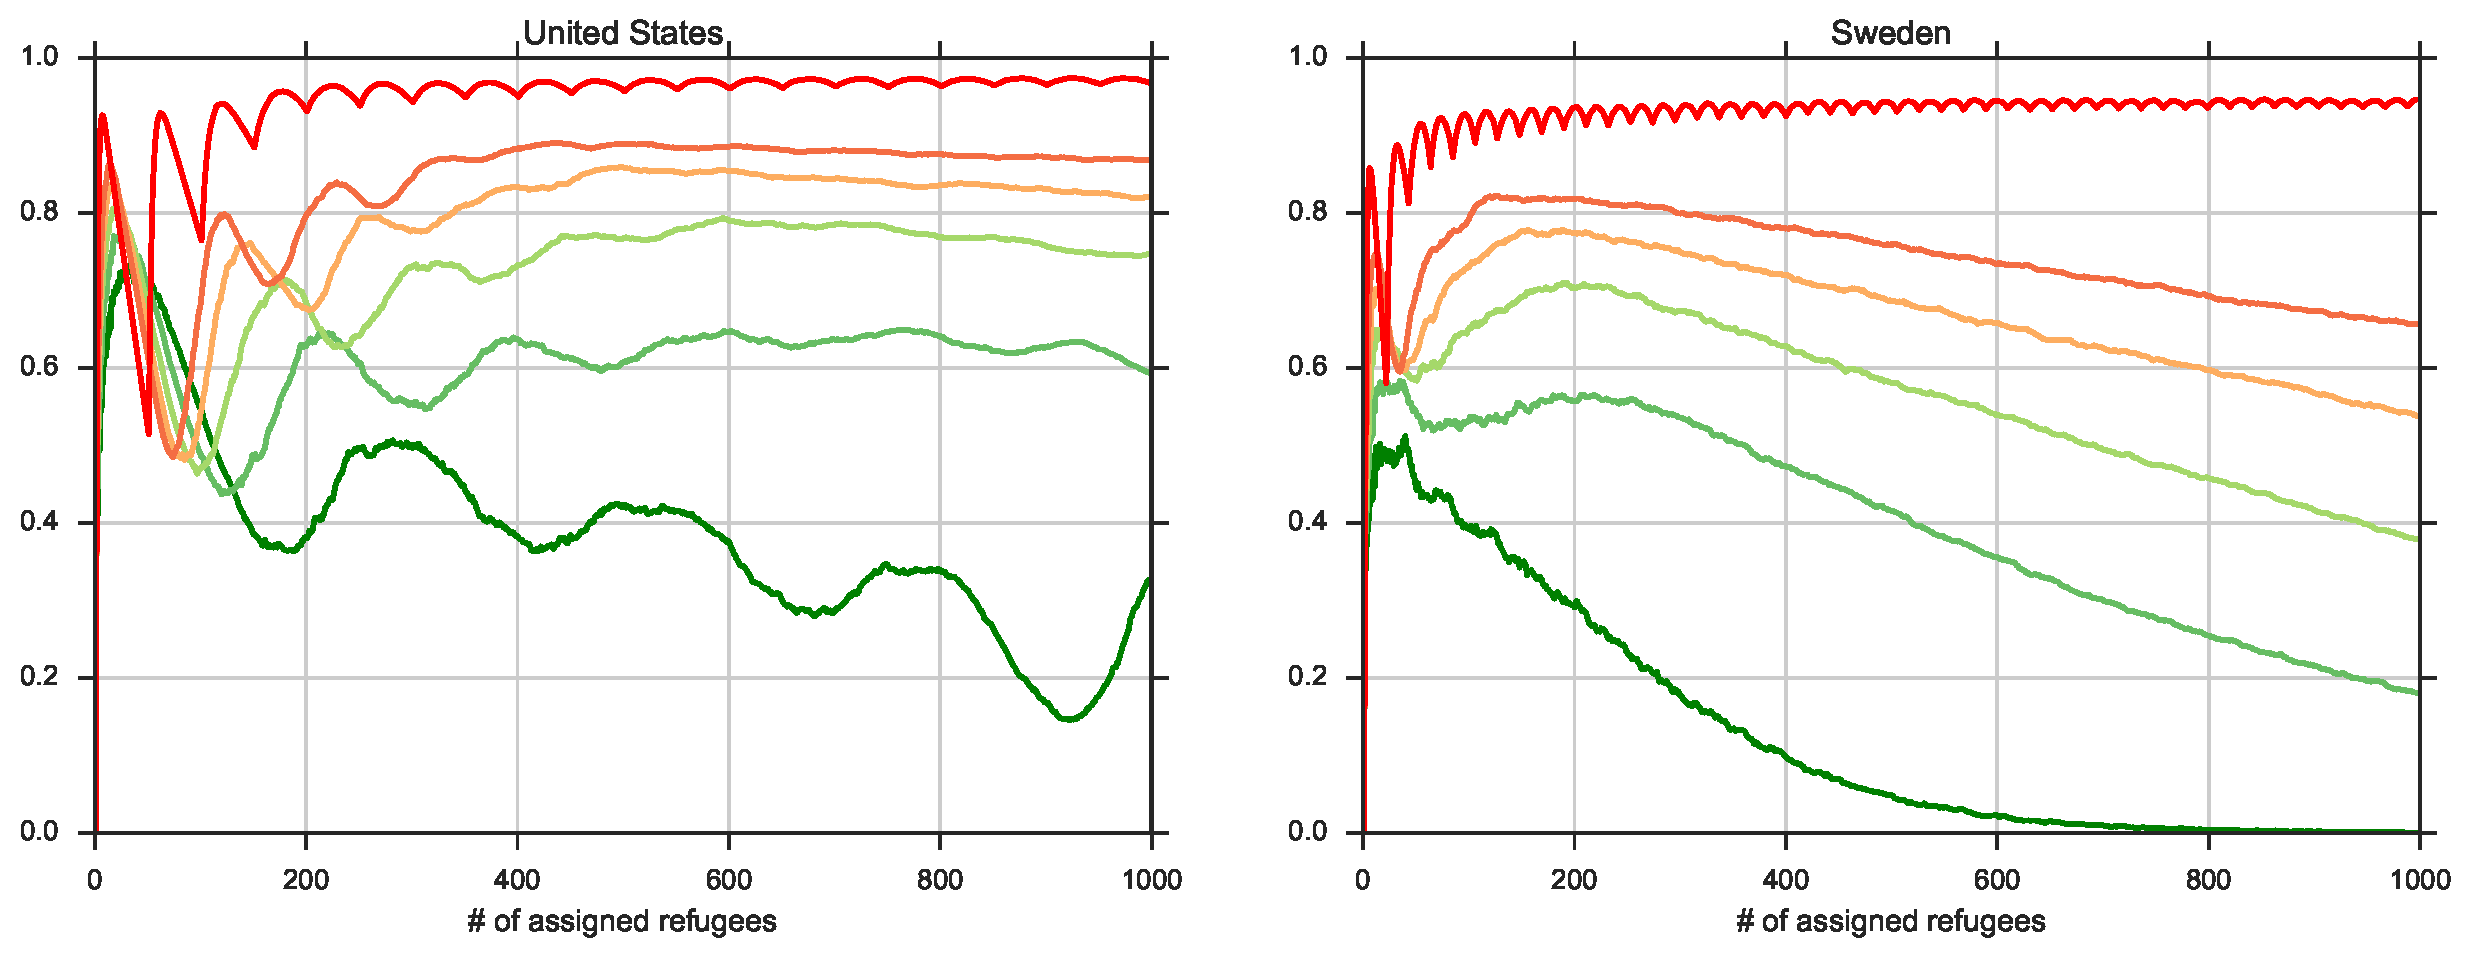
\includegraphics[width=\linewidth]{double_fair0_new.png}}
	\vspace{-0.7em}
	\subfloat[Share of localities envying some locality by at least five asylum seekers \label{SUBFIG-misclassification_fair1}]{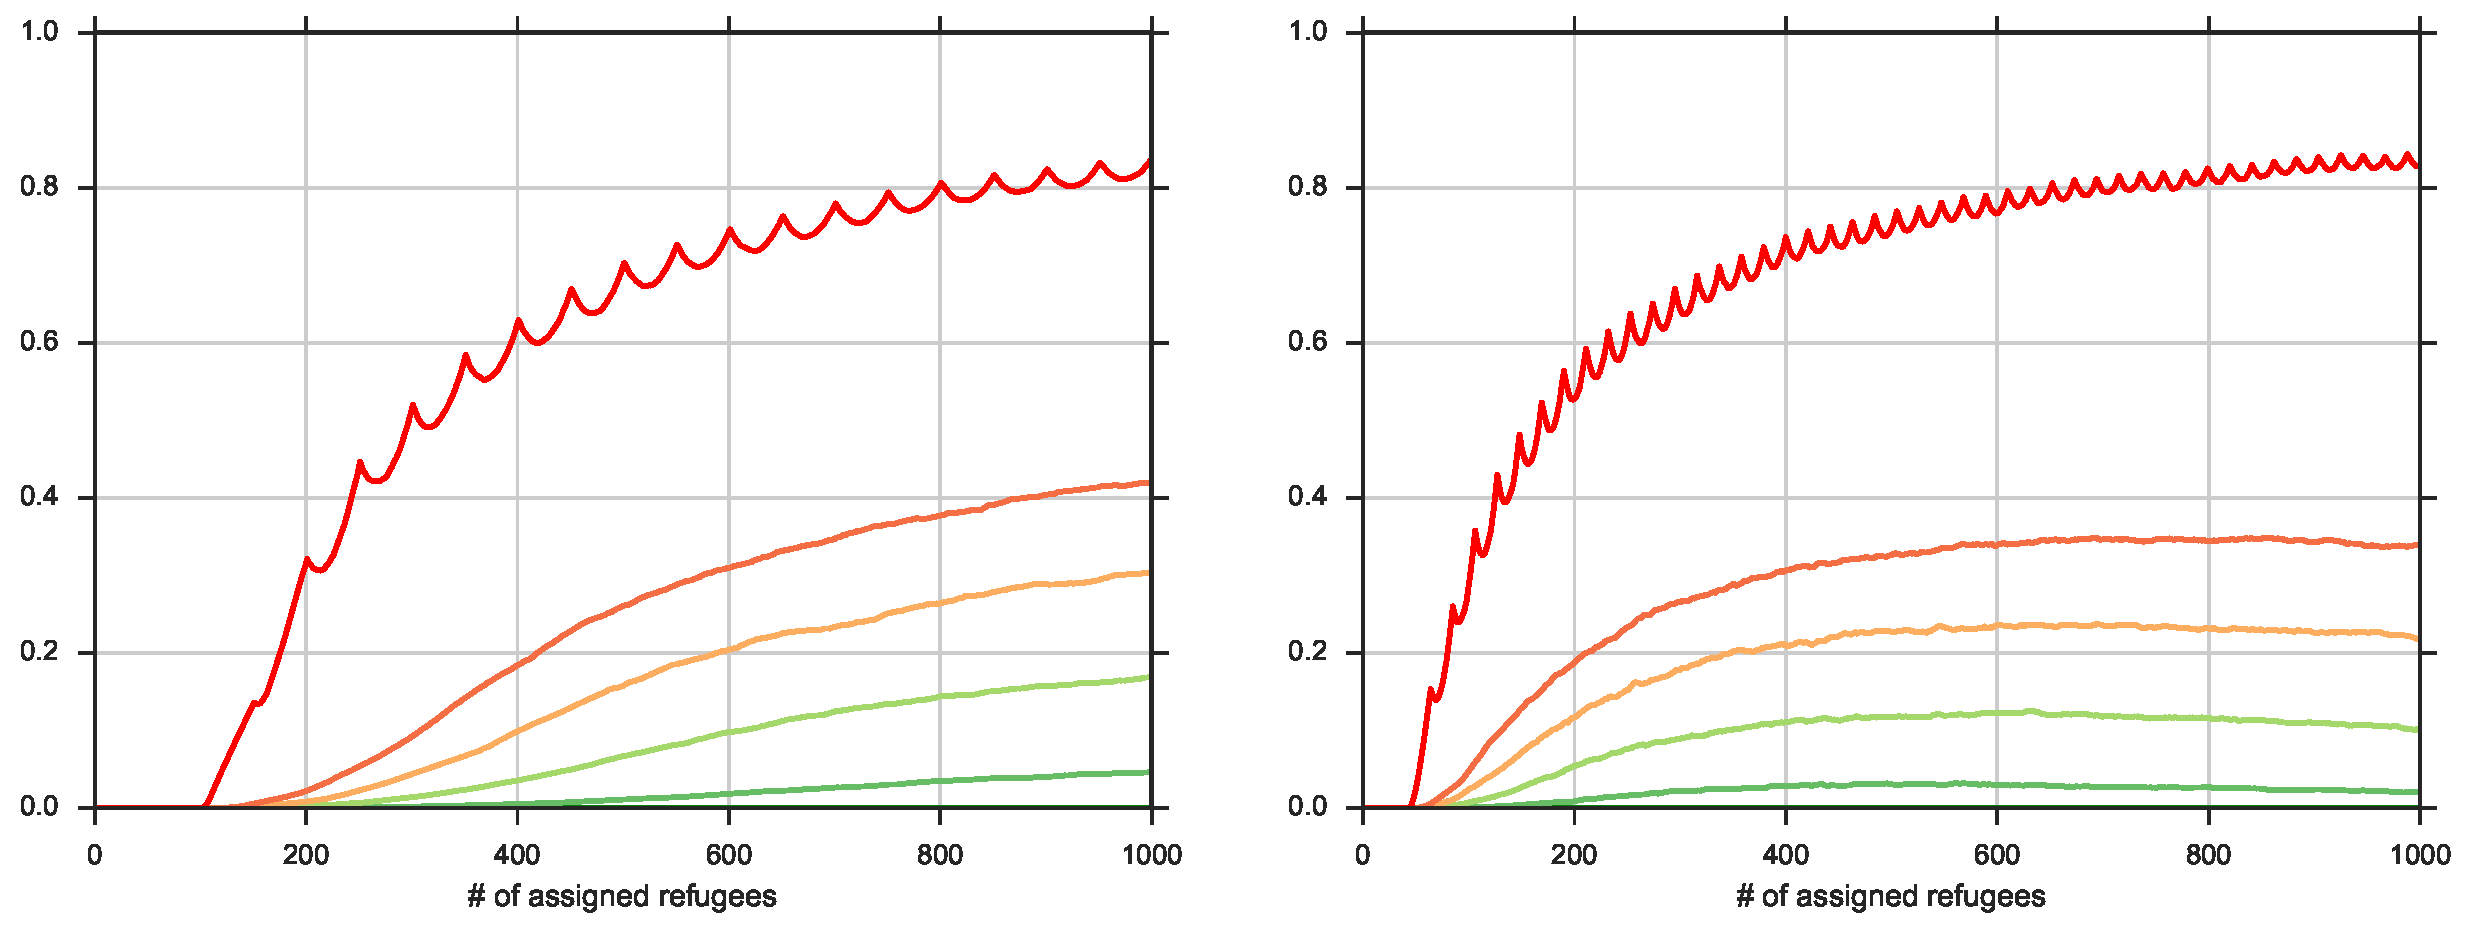
\includegraphics[width=\linewidth]{double_fair1_new.png}}
	\vspace{-0.7em}
	\subfloat[Share of mismatched acceptable asylum seekers \label{SUBFIG-misclassification_effic}]{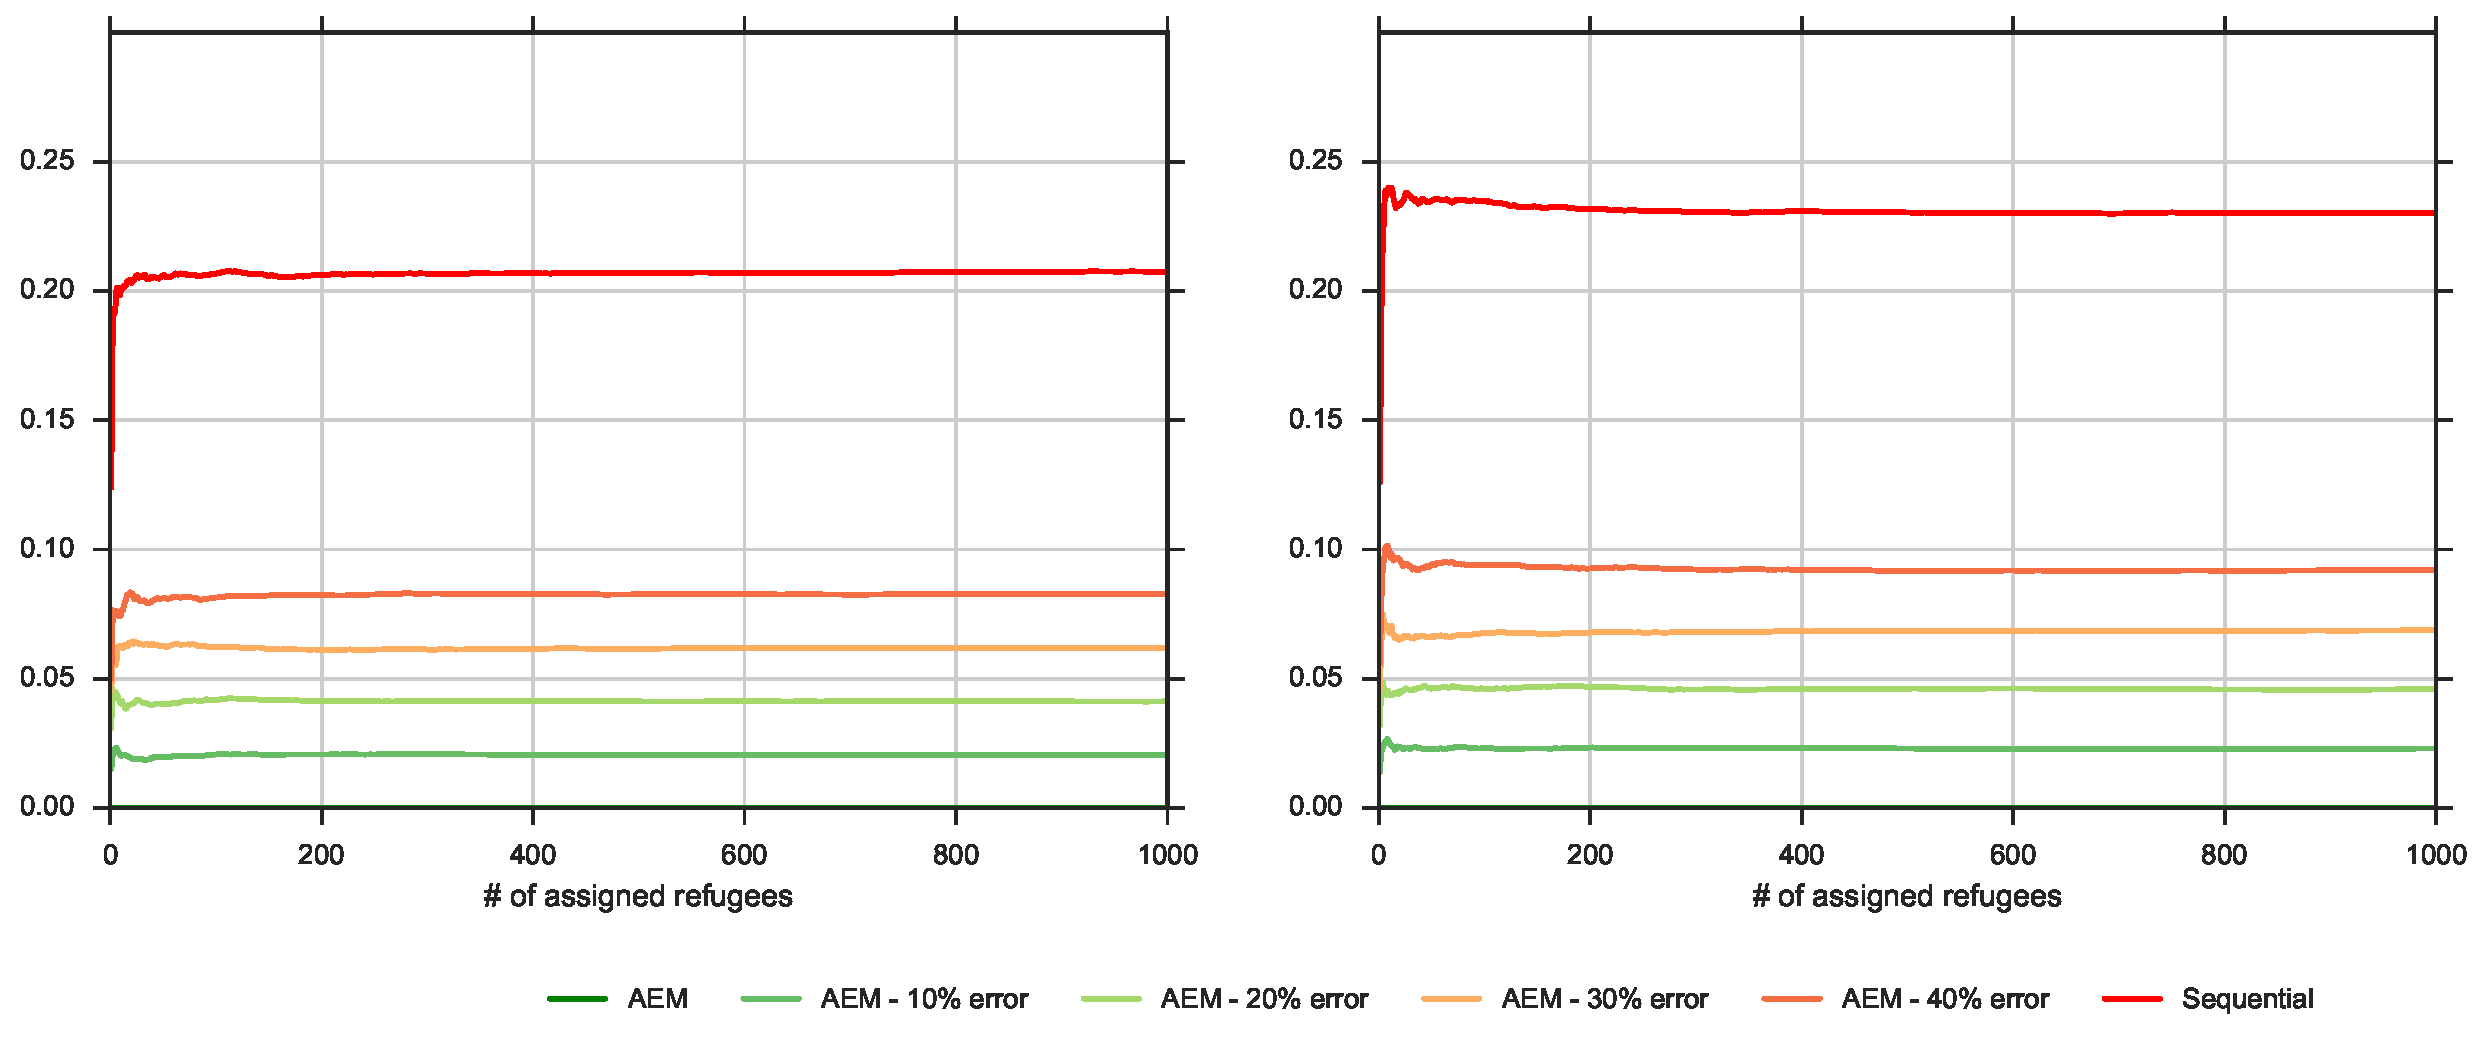
\includegraphics[width=\linewidth]{double_effic_new.png}}

	{\scriptsize \vspace{-1em}
	\begin{singlespace}
		{\sc Notes:} A thousand waves of asylum seekers of 1,000 asylum seekers each is simulated, distributed across 51 locations in the United States and the 21 Swedish regional entities (l{\"a}n). The measures of efficiency and envy is computed at each matching, comparing the performance of the proposed mechanism (with increasing degrees of misclassification error) with that of the na\"{i}ve sequential matching mechanism. The flows of asylum seekers are calibrated to match the numbers reported by \cite{bib:BansakEtAl} for the United States ($\overline{D}$: 34 percent; $\underline{D}$: 39 percent) and average 2016 employment outcomes of the 2013 asylum seeker wave in Sweden ($\overline{D}$: 28 percent; $\underline{D}$: 45 percent).
	\end{singlespace}
	 }
\end{figure}

Figure \ref{FIG-miclassification} compares the performance of the proposed mechanism (AEM) with increasing degrees of misclassification error in the locality-specific partitions with that of the na\"{i}ve sequential matching mechanism, in terms of both envy and efficiency. The proportion of localities in the sample envying some locality by at least one and at least five asylum seekers are used as measures of envy. If the locality-specific partitions are correct, Theorem \ref{THEOREM:envy_efficiency} shows that the proposed mechanism guarantees that envy is bounded by a single asylum seeker. Remarkably, Panel \ref{SUBFIG-misclassification_fair0} shows that the share of localities envying another locality by at least one asylum seeker decreases with the number of asylum seekers per locality, and converges towards zero. Even with misclassification error, Panels \ref{SUBFIG-misclassification_fair0} and \ref{SUBFIG-misclassification_fair1} in Figure \ref{FIG-miclassification} show that the proposed matching mechanism always outperforms the na\"{i}ve sequential matching mechanism in terms of envy. With the 24 percent misclassification error of \cite{bib:BansakEtAl}, the proposed mechanism guarantees decrease in envy of between 17 and 50 percent already after 1,000 arrivals (here it should be noted that there was around 25,000 asylum seekers in Sweden in 2016 and 2017).

Efficiency is measured as the share of asylum seekers that, while acceptable for some localities, end up in a locality that considers them unacceptable. This measure reflects the preferences of asylum seekers of achieving the best possible outcomes for their future, and is in a Pareto efficient matching always equal to zero. Even with misclassification error, the proposed mechanism produces strong efficiency gains with respect to the na\"{i}ve sequential matching mechanism. With the 24 percent misclassification error of \cite{bib:BansakEtAl}, the proposed mechanism decreases the share of mismatched acceptable asylum seekers by around 75 percent already after 1,000 arrivals.

\subsection{Choice of Quotas}\label{SEC:quotas}
The presence of heterogeneous quotas across localities introduces a further seasonality-related concern. For example, in Sweden each locality has the obligation by law of reserving housing units to asylum seekers \citep[Swedish Law,][]{SFS2016}. Yearly quotas coupled with the proposed mechanism will lead to that smaller localities will fill up all their housing obligation in a few months, and thus will be obliged to provide housing units only at a given time of the year. Larger localities will instead have to provide housing throughout the year. A solution to this disparity would be splitting yearly quotas in, e.g., trimester quotas, and dynamically match asylum seekers within each trimester. This section shows that such strategy is feasible and, as with random flows of asylum seekers, the performance of the proposed mechanism does not suffer from partitioning quotas across shorter time periods, and can actually improve for small enough misclassification error in the partition.

A thousand random flows of asylum seekers is simulated and calibrated as in Figure \ref{FIG-miclassification} for Sweden using the 2017 quotas.\footnote{These quotas are available at the website of the Swedish Migration Board, \texttt{www.migrationsverket.se}.} For each flow of asylum seekers, the quotas are splitted up at yearly, semestral, trimestral and monthly intervals.\footnote{In 2017, the sum of all quotas was 23,600. For simplicity, each yearly regional quota is rounded to a number divisible by 12, and thus flows of 23,568 asylum seekers are considered.} At each interval, the matching mechanism restarts either blindly (i.e., resetting the aggregated envy to at zero at the start of the considered period) or taking into account dynamic legacies (i.e., initiating the mechanism with the computed envy at the end of the previous period). The measures of envy and efficiency are compared at the end of the year, when the flow of asylum seekers has been completely assigned, and benchmark the results to those obtained through the na\"{i}ve sequential matching mechanism.

\begin{figure}
	\caption{Share of mismatched acceptable asylum seekers over quotas period \label{FIG-quotas}}
	\begin{center}
	\subfloat[No misclassification error \label{SUBFIG-quotas_fair0}]{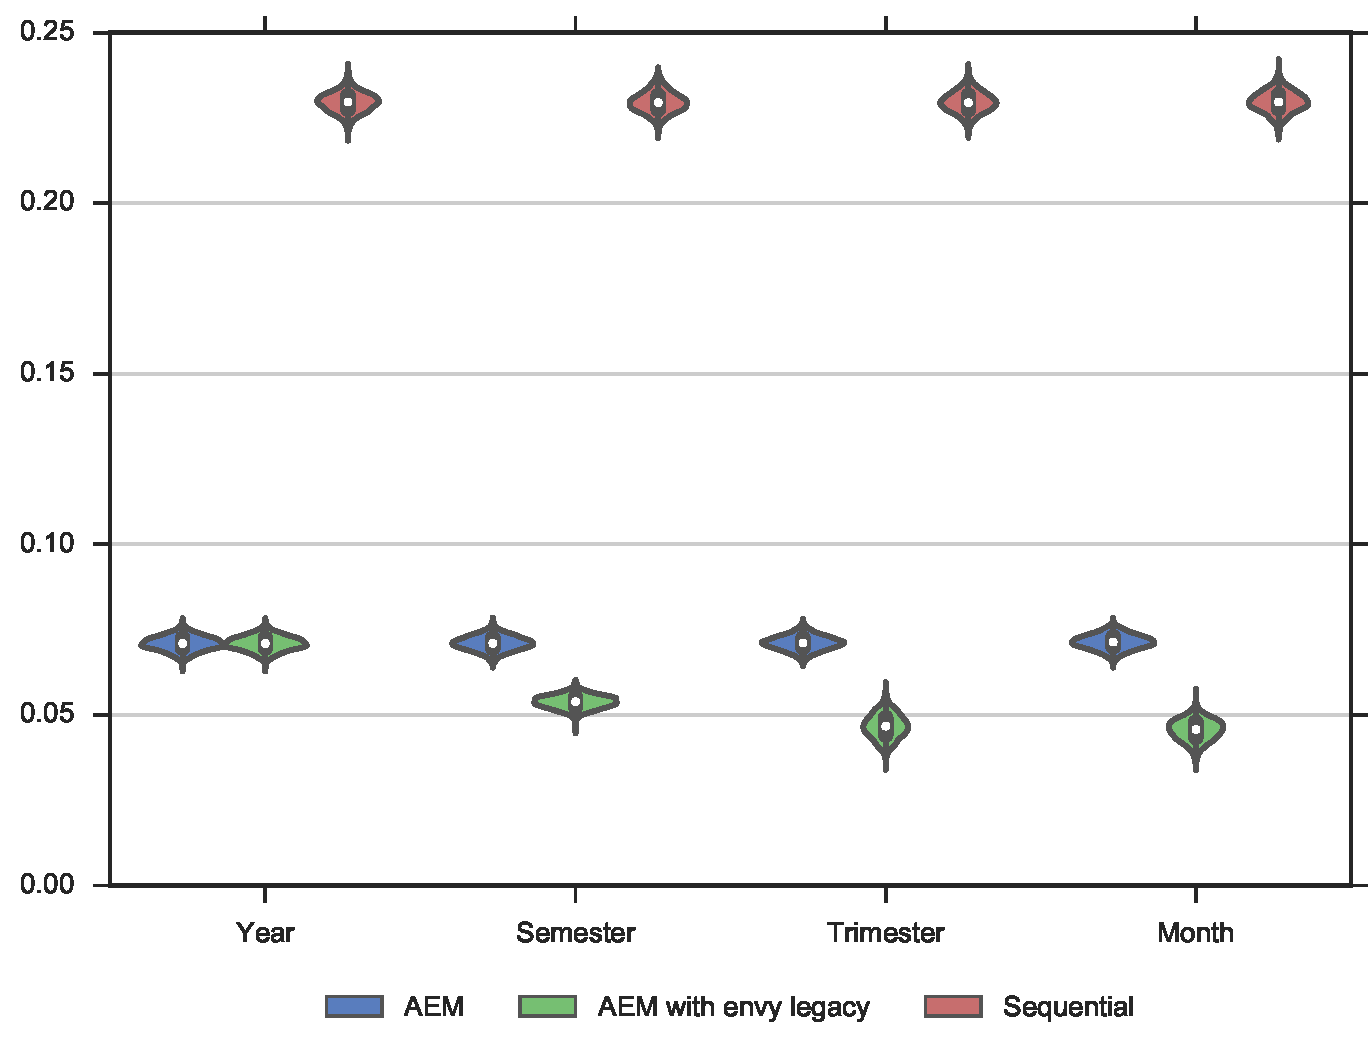
\includegraphics[width=0.5\linewidth]{single_effic_0_new.png}}
	\subfloat[24\% misclassification error \label{SUBFIG-quotas_effic}]{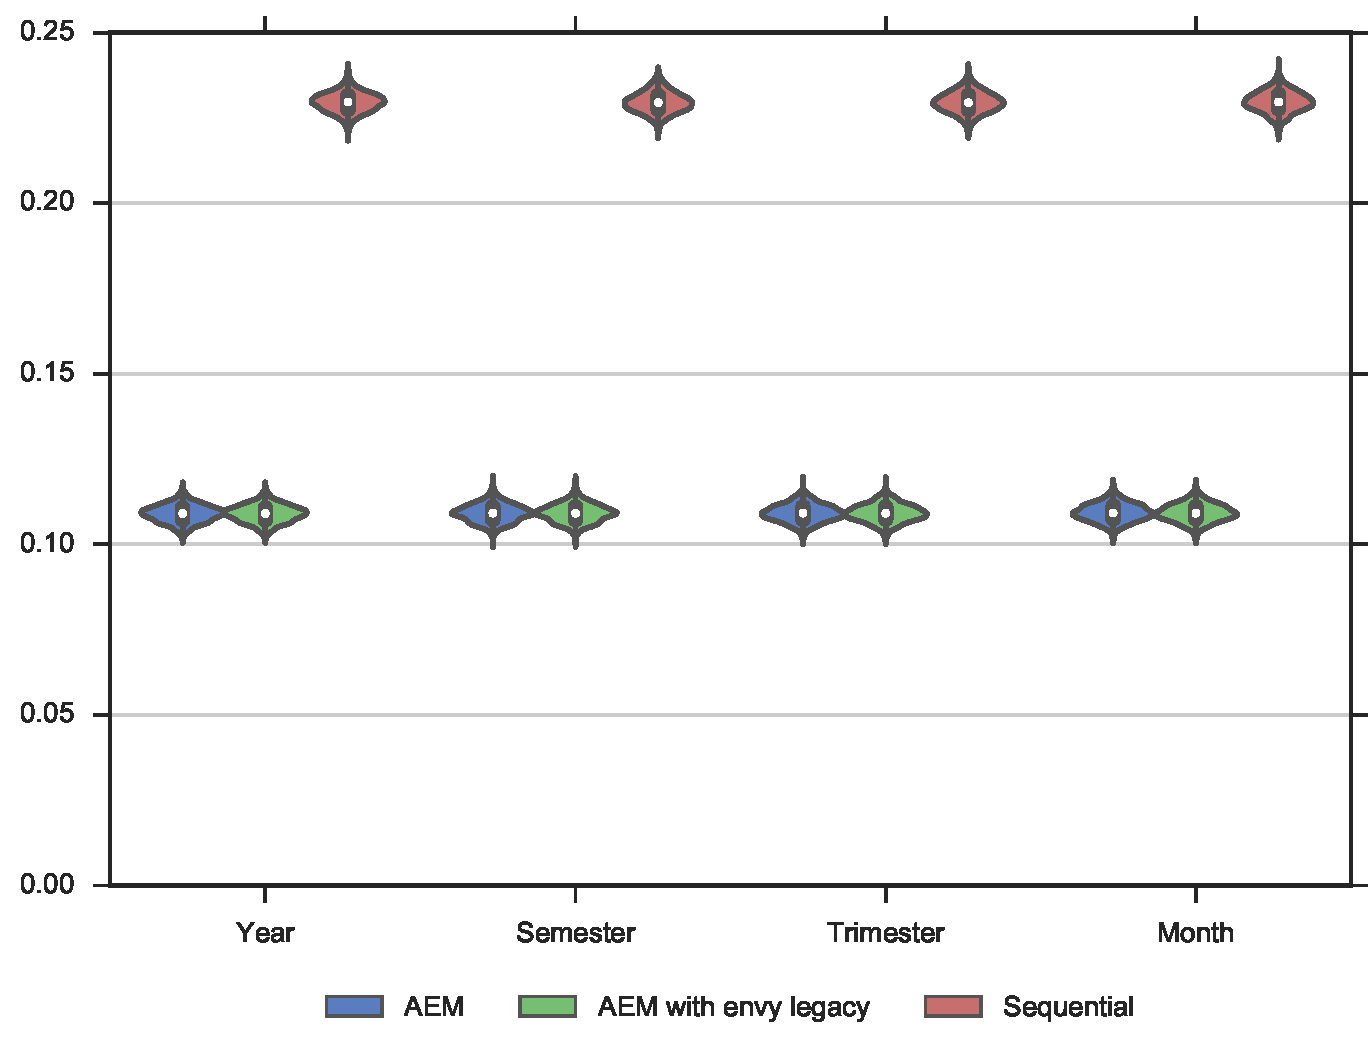
\includegraphics[width=0.5\linewidth]{single_effic_24_new.png}}
	\end{center}
		{\scriptsize \vspace{-1em}
	\begin{singlespace}
		{\sc Notes:} A thousand waves 23,568 asylum seekers each is simulated, distributed across 21 Swedish regional entities (l\"{a}n) according to 2017 Swedish regional quotas. The figure reports the distributions of efficiency measures calculated after the assignment of the 23,568th asylum seeker for (i) the proposed mechanism restarted blindly, (ii) the proposed mechanism allowing for envy legacy across sub-periods, and (iii) the na\"{i}ve sequential matching mechanism. Flows of asylum seekers are calibrated to match average 2016 employment outcomes of the 2013 asylum seeker wave in Sweden ($\overline{D}$: 28 percent; $\underline{D}$: 45 percent). Autocorrelation of locality preferences is allowed for each asylum seeker.
	\end{singlespace}
	 }
\end{figure}

Figure \ref{FIG-quotas} shows the distributions of the efficiency measure (the share of acceptable asylum seekers matched to a locality that finds them not acceptable) by matching mechanism and quota periods at completion of the yearly flow of asylum seekers.\footnote{Splitting quotas has no discernible effect on envy measures. These results appear in Appendix B.} With binding quotas, this measure can be different than zero even in absence of misclassification error, as it might happen that an asylum seeker would be acceptable, but only for localities that already exhausted their quotas. Nonetheless, independently on misclassification error, the proposed matching mechanism severely outperforms the na\"{i}ve sequential matching mechanism even in the presence of quotas, and partitioning quotas across shorter periods of time never harms its performance.

Moreover, with random flows of asylum seekers and no misclassification error, transmitting information on envy across across periods can allow partitioning quotas across shorter periods of time to increase match efficiency. Intuitively, this result is due to the matching mechanism placing envying localities earlier in the priority list and further down in the rejection list. As a consequence, envying small localities pick acceptable asylum seekers first (and thus fill their quotas primarily with asylum seekers in the sets $\overline{D}$ and $D$) as a compensation for missing out acceptable asylum seekers while excluded from the economy. However, if enough misclassification error is present, the mechanism does not realize that some small localities carry some envy across periods, and thus fail to compensate them and thereby improve the match efficiency.

\section{Conclusions}\label{SEC:conclusions}
This paper investigates dynamic refugee matching as a market design application. A specific matching mechanism was proposed and it has been demonstrated that any matching selected by the proposed mechanism is Pareto efficient and satisfies envy bounded by a single asylum seeker. This theoretical finding hinges on the assumption that there is no misclassification error. For example, \cite{bib:BansakEtAl} report 24 percent misclassification error for their preferred refugee assignment models estimated on US data. However, even with a 24 percent misclassification error, the proposed mechanism (i) decreases the share of mismatched acceptable asylum seekers by around 75 percent and (ii) guarantees a reduction in envy of between 17 and 50 percent.

This paper does not empirically estimate prediction functions, as we currently don't have access to to the necessary data. By exploiting refugee data from the United States and Switzerland, \cite{bib:BansakEtAl} estimate locality-specific partitions by a machine learning algorithm, allowing for locality-specific synergies with heterogeneous refugees. Because their algorithm focuses on minimizing prediction error rather than uncovering structural parameters determining labor market success \citep{bib:MullainathanSpiess}, machine learning is a particularly appropriate tool in this context. Such an unstructured approach highlights the low external validity of the estimated prediction function, which therefore needs to be re-estimated and re-calibrated in different scenarios and as new data becomes available. The necessity to update the prediction function has the benefit of alleviating the problem of displacement and general equilibrium effects due to the field implementation of mechanisms as the one proposed in this paper \citep{bib:CreponEtAl}. If the labor demand for asylum seekers is very inelastic, then even an efficient assignment does not guarantee employment for asylum seekers predicted as acceptable. In practice, this mismatch would increase prediction error in our predictions. However, re-estimating the prediction function with updated data would capture these effects and return a better predicted ``demand matrix'' in a later stage. 

A more theoretical remark is that the proposed mechanism assumes that asylum seekers arrive one-by-one. This means that the current form of the mechanism does not take families of asylum seekers into account \citep[see, e.g.,][for a mechanism that keeps families intact in house allocation problems with asylum seekers]{bib:AnderssonEhlers}. To also account for families, each asylum seeker can be described to be of a specific size representing the number of family members and some flexibility in the quotas must be allowed. In this case, envy cannot be guaranteed to be bounded by a single asylum seeker but is instead bounded by the maximal size of any family of asylum seekers in the sequence.

Finally, this paper has abstracted from issues related to manipulability. It is  well-established in the mechanism design literature that agents (localities in this paper) often cannot be prevented from manipulating mechanisms in their advantage by misrepresenting preferences. In the framework investigated in this paper, this means that localities may gain by classifying an acceptable asylum seeker as unacceptable or vice versa. To analyze this type of strategic behavior, some notion of dynamic (non-)manipulability needs to be introduced. Such analysis is beyond the scope of this paper. Furthermore, because the preferences exploited in this paper are derived from estimation not first-party reports, manipulability is unlikely to constitute a major problem in the considered dynamic refugee matching problem.


\section*{Appendix A: Proofs}
This Appendix contains the proofs of all results in the paper.

\medskip

\noindent\textbf{Proof of Theorem \ref{THEOREM:envy_efficiency}.} To prove Part (i) of the theorem, suppose that envy not is bounded by a single asylum seeker at matching $x(k)$. This means that there are two localities in $M(k)$, say $m$ and $m^\prime$, and two integers, say $k^0$ and $k^1$ (where $0<k^0<k^1\leq k$), such that:
\begin{itemize}
\item[(I)] locality $m$ is indifferent between bundles $x_{m}(k^0-1)$ and $x_{m^\prime}(k^0-1)$,
\item[(II)] locality $m$ envies locality $m^\prime$ by exactly one asylum seeker at matching $x(k^0)$, and
\item[(III)] locality $m$ envies locality $m^\prime$ by exactly two asylum seekers at matching $x(k^1)$.
\end{itemize}
\noindent Let $k^0$ and $k^1$ be the largest and the smallest integers, respectively, that satisfies (I)--(III), and consider the subsequence of $S$ containing the asylum seekers $S(k^0),\ldots,S(k^1)$. Because the integers $k^0$ and $k^1$ are chosen in the above way, locality $m$ has not been matched to any asylum seekers in the subsequence $S(k^0+1),\ldots,S(k^1-1)$, and locality $m^\prime$ has not been matched to any non-demanded asylum seeker or any asylum seeker that is acceptable for locality $m$ in the subsequence $S(k^0+1),\ldots,S(k^1-1)$. Hence, there may be four different reasons to why conditions (I)--(III) hold:
\begin{itemize}
\item[(a)] Asylum seekers $S(k^0)$ and $S(k^1)$ are acceptable to locality $m$ but are both matched to locality $m^\prime$,
\item[(b)] Asylum seeker $S(k^0)$ is non-demanded but matched to locality $m$ and asylum seeker $S(k^1)$ is acceptable to locality $m$ but matched to locality $m^\prime$,
\item[(c)] Asylum seeker $S(k^0)$ is acceptable to locality $m$ but matched to locality $m^\prime$ and asylum seeker $S(k^1)$ is non-demanded but matched to locality $m$,
\item[(d)] Asylum seekers $S(k^0)$ and $S(k^1)$ are non-demanded but are both matched to locality $m$.
\end{itemize}
\noindent It is only proved that parts (a) and (b) cannot hold as the corresponding proofs of parts (c) and (d) are almost identical. In the remaining part of this proof, it is assumed that asylum seeker $S(k^0)$ is of type $t^\prime$ and that asylum seeker $S(k^1)$ is of type $t^{\prime\prime}$.

To prove that (a) cannot hold, note that asylum seeker $S(k^0)$ is acceptable for both locality $m$ and $m^\prime$. Because of this and rotation, it also follows that locality $m^\prime$ has a higher priority than locality $m$ in $\pi_{t^\prime}(k^0)$ and the lowest priority in $\pi_t(k^0+1)$ for each $t\in T$. Because asylum seeker $S(k^1)$ is matched to locality $m^\prime$, it must also be the case that locality $m^\prime$ has a higher priority than locality $m$ in $\pi_{t^{\prime\prime}}(k^1)$. The latter can, however, not occur. To see this, recall first that locality $m$ not is matched any asylum seeker in the subsequence $S(k^0),\ldots,S(k^1)$. Hence, it cannot be the case that $m^\prime$ has a higher priority than locality $m$ in $\pi_{t^{\prime\prime}}(k^1)$ because locality $m$ is matched an asylum seeker. The reason must then be that locality $m^\prime$ is matched a non-demanded asylum seeker since this is the only way for locality $m^\prime$ to obtain a higher priority than $m$. But this contradicts the above conclusion that locality $m^\prime$ has not been matched any non-demanded asylum seeker in the subsequence $S(k^0+1),\ldots,S(k^1-1)$. Hence, (a) cannot hold.

To prove that condition (b) cannot hold, recall that asylum seeker $S(k^0)$ is non-demanded and that locality $m$ envies locality $m^\prime$ at matching $x(k^0)$. Because of this and rotation, it also follows that locality $m$ has a higher priority than locality $m^\prime$ in $\pi_t(k^0+1)$ for each $t\in T$. Because the overdemanded asylum seeker $S(k^1)$ is matched to locality $m^\prime$, it must be the case that locality $m^\prime$ has a higher priority than locality $m$ in $\pi_{t^{\prime\prime}}(k^1)$. The latter can, however, not occur due to the rules of the mechanism. To see this, recall first that locality $m$ not is matched any asylum seeker in the subsequence $S(k^0),\ldots,S(k^1)$. Hence, it cannot be the case that $m^\prime$ has a higher priority than locality $m$ in $\pi_{t^{\prime\prime}}(k^1)$ because locality is matched to an asylum seeker. The reason must then be that locality $m^\prime$ is matched to a non-demanded asylum seeker since this is the only way for locality $m^\prime$ to obtain a higher priority than $m$. But this contradicts the above conclusion that locality $m^\prime$ has not been matched to any non-demanded asylum seeker in the subsequence $S(k^0+1),\ldots,S(k^1-1)$.

To prove Part (ii) of the theorem, suppose that $x(k)$ not is Pareto efficient. Consider next the localities in the set $M(k)$ and the asylum seekers in the set $A(k)$. Because $x(k)$ not is Pareto efficient, by assumption, there exists an matching $x^\prime(k)$ where the quotas are respected for all localities in $M(k)$, $x_m^\prime(k)R_m(k) x_m(k)$ for all $m\in M(k)$, and $x_m^\prime(k)P_m(k) x_m(k)$ for some $m\in M(k)$. The latter conditions imply that:
\begin{equation}
\sum_{j\in M(k)}\left(|A_j^+(x_j^\prime)|-|A_j^-(x_j^\prime)|\right)>\sum_{j\in M(k)}\left(|A_j^+({x_j})|-|A_j^-({x_j})|\right).\label{EQ:not_efficient_A}
\end{equation}
\noindent Note next that a locality in $M(k)$ can only be matched to an unacceptable asylum seeker if the asylum seeker also is unacceptable for all other localities in $M(k)$. This follows since $\varphi$ is a structure mechanism. But this also means that $\sum_{j\in M(k)}|A_j^-(x_j^\prime)|=\sum_{j\in M(k)}|A_j^-({x_j})|$. Consequently, condition (\ref{EQ:not_efficient_A}) reduces to:
\begin{equation}
\sum_{j\in M(k)}|A_j^+(x_j^\prime)|>\sum_{j\in M(k)}|A_j^+({x_j})|,\label{EQ:not_efficient_B}
\end{equation}
\noindent i.e., that the total number of acceptable asylum seekers matched to the localities in $M(k)$ is greater at matching $x^\prime(k)$ than at matching $x(k)$. But this is not possible since all asylum seekers in $A(k)$ are matched to some locality in $M(k)$ which finds them acceptable by construction of the structure mechanism $\varphi$. Hence, $x(k)$ must be Pareto efficient. \hfill $\square$

\medskip

\noindent\textbf{Proof of Theorem \ref{TH:structures}.} Only the first part of the statement is proved since the second part of the theorem is based on symmetrical arguments. In the remaining part of the proof, it is assumed that asylum seeker $S(k)$ is of type $t\in T$. For convenience, it is also, without loss of generality, written $\pi_t(k)$ in the remaining part of this proof instead of the formally correct statement ``$\pi_t(k)$ for each $t\in T$''.

The result is proved by induction. It is first demonstrated that the result is true for $\pi_t(2)$. Three cases must be considered:

\begin{itemize}

\item[(1.a)] Asylum seeker $S(1)$ is non-demanded. Because $S(1)$ not is demanded by any locality in $M(1)$, no
locality in $M(1)$ will envy the locality that is matched to $S(1)$ and the locality that is
matched to $S(1)$ will envy all localities in $M(1)$. Because the structure $(\pi(1),\sigma(1))$ satisfies
rotation, the locality that is matched to $S(1)$ will have the highest priority in $\pi_t(2)$. These arguments
show that no locality in $M(1)$ envies any locality with a higher priority in $\pi_t(2)$.

\item[(1.b)] Asylum seeker $S(1)$ is demanded. In this case, $S(1)$ is matched to the only locality that demands
$S(1)$ and no locality will envy this locality. Similarly, the locality that is matched to $S(1)$ will also not envy any other locality since $S(1)$ is acceptable. Because the structure $(\pi(1),\sigma(1))$ satisfies rotation,
it follows that $\pi_t(1)=\pi_t(2)$, and, consequently, no locality in $M(1)$ envies any
locality with a higher priority in $\pi_t(2)$.

\item[(1.c)] Asylum seeker $S(1)$ is overdemanded. $S(1)$ is matched to the locality in $M(1)$ with the highest
priority in $\pi_t(1)$ that finds asylum seeker $S(1)$ acceptable. This locality will be envied by all
localities that find $S(1)$ acceptable and the locality that is matched to $S(1)$ will not envy any
locality in $M(1)$. Because the structure $(\pi(1),\sigma(1))$ satisfies rotation, the
locality that is matched to $S(1)$ will have the lowest priority in $\pi_t(2)$. These arguments show that no
locality in $M(1)$ envies any locality with a higher priority in $\pi_t(2)$.

\end{itemize}

\noindent From the above arguments, we conclude that the statement is true for $\pi_t(2)$. Consider now the
induction assumption that the result holds for $\pi_t(k)$ for an arbitrary $k\in \{2,\ldots,S-1\}$. Given this
assumption, it remains to show that the result is true for $\pi_t(k)$. Again, three cases must be considered:

\begin{itemize}

\item[(k.a)] Asylum seeker $S(k)$ is non-demanded. Because $S(k)$ not is demanded by any locality in $M(k)$
and because envy is bounded by a single asylum seeker at matching $x(k-1)$ by Theorem \ref{THEOREM:envy_efficiency}, no
locality in $M(k)$ will envy the locality that is matched to $S(k)$ at matching $x(k)$. Because the structure
$(\pi(k),\sigma(k))$ satisfies rotation, the locality that is matched to $S(k)$ will have a higher priority
in $\pi_t(k+1)$ than all localities that the locality envies at matching $x(k)$. These arguments show that
no locality in $M(k)$ envies any locality with a higher priority in $\pi_t(k+1)$.

\item[(k.b)] Asylum seeker $S(k)$ is demanded. In this case, $S(k)$ is matched to the only locality that demands
$S(k)$. Because the structure $(\pi(k),\sigma(k))$ satisfies rotation, it must be the case that $\pi_t(k)=\pi_t(k+1)$. Consequently, the result holds for $\pi_t(k+1)$ since the result is true for $\pi_t(k)$ by the induction assumption.

\item[(k.c)] Asylum seeker $S(k)$ is overdemanded. $S(k)$ is matched to the locality in $M(k)$ with the highest
priority in $\pi(k)$ that finds asylum seeker $S(k)$ acceptable. Because envy is bounded by a single asylum seeker
at matching $x(k-1)$ by Theorem \ref{THEOREM:envy_efficiency}, the locality that is matched to the acceptable asylum seeker $S(k)$ will
not envy any locality at matching $x(k)$. Then because the structure $(\pi(k),\sigma(k))$ satisfies rotation,
the locality that is matched to $S(k)$ will have the lowest priority in $\pi_t(k+1)$. But then result holds by the above arguments.

\end{itemize}

\noindent The above three cases, together with the result for $\pi_t(2)$ and the induction assumption, proves that
locality $m$ does not envy any locality with a higher priority in $\pi_t(k)$. \hfill $\square$

\medskip

\noindent\textbf{Proof of Corollary \ref{COROLLARY:envy}.} Because matching $x(k)$ is selected by $\varphi$, it follows from Theorem \ref{THEOREM:envy_efficiency} that envy for locality $m$ towards locality $m^\prime$ is bounded by a single asylum seeker, i.e., that:
\begin{equation}
A_m^+(x_m(k))-A_m^-(x_m(k))+1\geq A_m^+(x_{m^\prime}(k))-A_m^-(x_{m^\prime}(k)).\label{EQ:COR_1}
\end{equation}
\noindent To obtain a contradiction, suppose now that the statement not is true. Then:
\begin{eqnarray}
&& A_m^+(x_{m^\prime}(k))>A_m^+(x_m(k)),\label{EQ:COR_2} \\
&& A_m^-(x_m(k))>A_m^-(x_{m^\prime}(k)).\label{EQ:COR_3}
\end{eqnarray}
\noindent Inequality (\ref{EQ:COR_2}) implies that $A_m^+(x_{m^\prime}(k))-1\geq A_m^+(x_m(k))$. This condition together with inequality (\ref{EQ:COR_1}) implies that $A_m^-(x_{m^\prime}(k))\geq A_m^-(x_m(k))$. But this inequality contradicts inequality (\ref{EQ:COR_3}).\hfill $\square$

\section*{Appendix B: Additional Simulation Results}
To be added in a future version of the paper.

\bibliographystyle{chicago}
\bibliography{ref}


\end{document}

